% Options for packages loaded elsewhere
\PassOptionsToPackage{unicode}{hyperref}
\PassOptionsToPackage{hyphens}{url}
%
\documentclass[
]{book}
\usepackage{amsmath,amssymb}
\usepackage{lmodern}
\usepackage{iftex}
\ifPDFTeX
  \usepackage[T1]{fontenc}
  \usepackage[utf8]{inputenc}
  \usepackage{textcomp} % provide euro and other symbols
\else % if luatex or xetex
  \usepackage{unicode-math}
  \defaultfontfeatures{Scale=MatchLowercase}
  \defaultfontfeatures[\rmfamily]{Ligatures=TeX,Scale=1}
\fi
% Use upquote if available, for straight quotes in verbatim environments
\IfFileExists{upquote.sty}{\usepackage{upquote}}{}
\IfFileExists{microtype.sty}{% use microtype if available
  \usepackage[]{microtype}
  \UseMicrotypeSet[protrusion]{basicmath} % disable protrusion for tt fonts
}{}
\makeatletter
\@ifundefined{KOMAClassName}{% if non-KOMA class
  \IfFileExists{parskip.sty}{%
    \usepackage{parskip}
  }{% else
    \setlength{\parindent}{0pt}
    \setlength{\parskip}{6pt plus 2pt minus 1pt}}
}{% if KOMA class
  \KOMAoptions{parskip=half}}
\makeatother
\usepackage{xcolor}
\usepackage{color}
\usepackage{fancyvrb}
\newcommand{\VerbBar}{|}
\newcommand{\VERB}{\Verb[commandchars=\\\{\}]}
\DefineVerbatimEnvironment{Highlighting}{Verbatim}{commandchars=\\\{\}}
% Add ',fontsize=\small' for more characters per line
\usepackage{framed}
\definecolor{shadecolor}{RGB}{248,248,248}
\newenvironment{Shaded}{\begin{snugshade}}{\end{snugshade}}
\newcommand{\AlertTok}[1]{\textcolor[rgb]{0.94,0.16,0.16}{#1}}
\newcommand{\AnnotationTok}[1]{\textcolor[rgb]{0.56,0.35,0.01}{\textbf{\textit{#1}}}}
\newcommand{\AttributeTok}[1]{\textcolor[rgb]{0.77,0.63,0.00}{#1}}
\newcommand{\BaseNTok}[1]{\textcolor[rgb]{0.00,0.00,0.81}{#1}}
\newcommand{\BuiltInTok}[1]{#1}
\newcommand{\CharTok}[1]{\textcolor[rgb]{0.31,0.60,0.02}{#1}}
\newcommand{\CommentTok}[1]{\textcolor[rgb]{0.56,0.35,0.01}{\textit{#1}}}
\newcommand{\CommentVarTok}[1]{\textcolor[rgb]{0.56,0.35,0.01}{\textbf{\textit{#1}}}}
\newcommand{\ConstantTok}[1]{\textcolor[rgb]{0.00,0.00,0.00}{#1}}
\newcommand{\ControlFlowTok}[1]{\textcolor[rgb]{0.13,0.29,0.53}{\textbf{#1}}}
\newcommand{\DataTypeTok}[1]{\textcolor[rgb]{0.13,0.29,0.53}{#1}}
\newcommand{\DecValTok}[1]{\textcolor[rgb]{0.00,0.00,0.81}{#1}}
\newcommand{\DocumentationTok}[1]{\textcolor[rgb]{0.56,0.35,0.01}{\textbf{\textit{#1}}}}
\newcommand{\ErrorTok}[1]{\textcolor[rgb]{0.64,0.00,0.00}{\textbf{#1}}}
\newcommand{\ExtensionTok}[1]{#1}
\newcommand{\FloatTok}[1]{\textcolor[rgb]{0.00,0.00,0.81}{#1}}
\newcommand{\FunctionTok}[1]{\textcolor[rgb]{0.00,0.00,0.00}{#1}}
\newcommand{\ImportTok}[1]{#1}
\newcommand{\InformationTok}[1]{\textcolor[rgb]{0.56,0.35,0.01}{\textbf{\textit{#1}}}}
\newcommand{\KeywordTok}[1]{\textcolor[rgb]{0.13,0.29,0.53}{\textbf{#1}}}
\newcommand{\NormalTok}[1]{#1}
\newcommand{\OperatorTok}[1]{\textcolor[rgb]{0.81,0.36,0.00}{\textbf{#1}}}
\newcommand{\OtherTok}[1]{\textcolor[rgb]{0.56,0.35,0.01}{#1}}
\newcommand{\PreprocessorTok}[1]{\textcolor[rgb]{0.56,0.35,0.01}{\textit{#1}}}
\newcommand{\RegionMarkerTok}[1]{#1}
\newcommand{\SpecialCharTok}[1]{\textcolor[rgb]{0.00,0.00,0.00}{#1}}
\newcommand{\SpecialStringTok}[1]{\textcolor[rgb]{0.31,0.60,0.02}{#1}}
\newcommand{\StringTok}[1]{\textcolor[rgb]{0.31,0.60,0.02}{#1}}
\newcommand{\VariableTok}[1]{\textcolor[rgb]{0.00,0.00,0.00}{#1}}
\newcommand{\VerbatimStringTok}[1]{\textcolor[rgb]{0.31,0.60,0.02}{#1}}
\newcommand{\WarningTok}[1]{\textcolor[rgb]{0.56,0.35,0.01}{\textbf{\textit{#1}}}}
\usepackage{longtable,booktabs,array}
\usepackage{calc} % for calculating minipage widths
% Correct order of tables after \paragraph or \subparagraph
\usepackage{etoolbox}
\makeatletter
\patchcmd\longtable{\par}{\if@noskipsec\mbox{}\fi\par}{}{}
\makeatother
% Allow footnotes in longtable head/foot
\IfFileExists{footnotehyper.sty}{\usepackage{footnotehyper}}{\usepackage{footnote}}
\makesavenoteenv{longtable}
\usepackage{graphicx}
\makeatletter
\def\maxwidth{\ifdim\Gin@nat@width>\linewidth\linewidth\else\Gin@nat@width\fi}
\def\maxheight{\ifdim\Gin@nat@height>\textheight\textheight\else\Gin@nat@height\fi}
\makeatother
% Scale images if necessary, so that they will not overflow the page
% margins by default, and it is still possible to overwrite the defaults
% using explicit options in \includegraphics[width, height, ...]{}
\setkeys{Gin}{width=\maxwidth,height=\maxheight,keepaspectratio}
% Set default figure placement to htbp
\makeatletter
\def\fps@figure{htbp}
\makeatother
\setlength{\emergencystretch}{3em} % prevent overfull lines
\providecommand{\tightlist}{%
  \setlength{\itemsep}{0pt}\setlength{\parskip}{0pt}}
\setcounter{secnumdepth}{5}
\usepackage{booktabs}
\usepackage{fontspec}
\usepackage{multirow}
\usepackage{multicol}
\usepackage{colortbl}
\usepackage{hhline}
\usepackage{longtable}
\usepackage{float}
\usepackage{wrapfig}
\usepackage{array}
\usepackage{hyperref}
\ifLuaTeX
  \usepackage{selnolig}  % disable illegal ligatures
\fi
\usepackage[]{natbib}
\bibliographystyle{plainnat}
\IfFileExists{bookmark.sty}{\usepackage{bookmark}}{\usepackage{hyperref}}
\IfFileExists{xurl.sty}{\usepackage{xurl}}{} % add URL line breaks if available
\urlstyle{same} % disable monospaced font for URLs
\hypersetup{
  pdftitle={Survey Design and Analysis},
  pdfauthor={Michael Foley},
  hidelinks,
  pdfcreator={LaTeX via pandoc}}

\title{Survey Design and Analysis}
\author{Michael Foley}
\date{2022-11-13}

\usepackage{amsthm}
\newtheorem{theorem}{Theorem}[chapter]
\newtheorem{lemma}{Lemma}[chapter]
\newtheorem{corollary}{Corollary}[chapter]
\newtheorem{proposition}{Proposition}[chapter]
\newtheorem{conjecture}{Conjecture}[chapter]
\theoremstyle{definition}
\newtheorem{definition}{Definition}[chapter]
\theoremstyle{definition}
\newtheorem{example}{Example}[chapter]
\theoremstyle{definition}
\newtheorem{exercise}{Exercise}[chapter]
\theoremstyle{definition}
\newtheorem{hypothesis}{Hypothesis}[chapter]
\theoremstyle{remark}
\newtheorem*{remark}{Remark}
\newtheorem*{solution}{Solution}
\begin{document}
\maketitle

{
\setcounter{tocdepth}{1}
\tableofcontents
}
\hypertarget{preface}{%
\chapter*{Preface}\label{preface}}
\addcontentsline{toc}{chapter}{Preface}

This is a compilation of notes from my study of survey design and analysis. I completed Data Camp courses \href{https://app.datacamp.com/learn/courses/survey-and-measurement-development-in-r}{Survey and Measurement Development in R} \citep{mount} and \href{https://app.datacamp.com/learn/courses/analyzing-survey-data-in-r}{Analyzing Survey Data in R} \citep{mcconville}, then moved on to Thomas Lumley's \href{http://r-survey.r-forge.r-project.org/svybook/}{Complex Surveys: a guide to analysis using R} \citep{lumley2010}. The following resources are also helpful.

\begin{itemize}
\tightlist
\item
  UCLA IDRE seminar \citep{idre}
\end{itemize}

\hypertarget{the-survey-package}{%
\section*{The survey Package}\label{the-survey-package}}
\addcontentsline{toc}{section}{The survey Package}

Only simple random sample survey designs can be analyzed with with normal statistical test functions - complex survey designs require special treatment. The \textbf{survey} package \citep{R-survey} handles both simple and complex survey designs. It contains a few data sets that will serve as examples in these notes. There is also a helper package named \textbf{jtools} \citep{R-jtools} that will come in handy for regression.

\begin{Shaded}
\begin{Highlighting}[]
\FunctionTok{library}\NormalTok{(tidyverse)}
\FunctionTok{library}\NormalTok{(survey)}
\FunctionTok{library}\NormalTok{(jtools)}

\FunctionTok{data}\NormalTok{(api, }\AttributeTok{package =} \StringTok{"survey"}\NormalTok{)}
\end{Highlighting}
\end{Shaded}

\hypertarget{common-terms}{%
\section*{Common Terms}\label{common-terms}}
\addcontentsline{toc}{section}{Common Terms}

Complex survey designs scale the \emph{n} data observations up to the \emph{N} population values. Each observation has an associated \emph{sampling weight}. A sampling weight is a \emph{probability weight} with on or more adjustments for non-response, non-coverage, calibration, and trimming.

For a \textbf{simple random sample}, the sampling weights equal the probability weights, \emph{N/n}, meaning each observation represents \emph{N/n} people.

In \textbf{stratified sampling}, the population is initially segmented by interesting factors (e.g.~gender, race/ethnicity, or SES), then sampled with simple random sampling. This ensures a specified number of observations for each stratum. The sample is less variable because the stratification process eliminates one source of variability. The sampling weights equal the probability weights again, but now there are separate weights for each stratum, \(N_A / n_A\), \(N_B / n_B\), etc.

\textbf{Cluster sampling} segments a population (usually geographically) into clusters, then randomly selects clusters to survey. Within a cluster, all members may be sampled (single stage design), or a random sample is taken (multi-stage design). Cluster sampling is almost universal in large-scale surveys involving in-person interviews because it dramatically reduces cost. Unfortunately, it also increases variance because observations within a cluster tend to me similar.

You will often encounter the term \emph{primary sampling unit} (PSU). It is the factor used for the initial sampling. For cluster sampling, it is the initial cluster; for stratified and simple random samples, it is the elementary unit.

A second term you will encounter is \emph{finite population correction}. It is a probability term that becomes relevant when the sampling fraction of the population becomes large. It equals \(\sqrt{(N-n)/(N-1)}\).

\hypertarget{survey-and-measurement-development}{%
\chapter{Survey and Measurement Development}\label{survey-and-measurement-development}}

A full survey project usually consists of six phases.

\begin{enumerate}
\def\labelenumi{\arabic{enumi}.}
\item
  \textbf{Item Generation}. Start by generating a list of candidate survey items. With help from SMEs, you evaluate the equivalence (interrater reliability) and content validity of the candidate survey items and pare down the list into the final survey.
\item
  \textbf{Survey Administration}. Administer the survey to respondents and perform an exploratory data analysis. Summarize the Likert items with plots and look for correlations among the variables.
\item
  \textbf{Item Reduction}. Explore the dimensions of the latent variable in the survey data with parallel analysis and exploratory factor analysis. Assess the internal consistency of the items with Cronbach's alpha and split-half tests, and remove items that do not add value and/or amend your theory of the number of dimensions.
\item
  \textbf{Confirmatory Factor Analysis}. Perform a formal hypothesis test of the theory that emerged from the exploratory factor analysis.
\item
  \textbf{Convergent/Discriminant Validity}. Test for convergent and discriminant construct validity.
\item
  \textbf{Replication}. Establish test-retest reliability and criterion validity.
\end{enumerate}

\hypertarget{background-quality}{%
\section{Background: Quality}\label{background-quality}}

\href{https://www.scribbr.com/methodology/reliability-vs-validity/}{Quality} surveys should be both \emph{reliable} (consistent) and \emph{valid} (accurate).

\hypertarget{reliability}{%
\subsection{Reliability}\label{reliability}}

A survey's reliability is the extent to which the results can be reproduced when repeated under similar conditions. You assess reliability three ways:

\begin{itemize}
\tightlist
\item
  \textbf{Equivalence (aka Interrater)}. Interrater reliability generally means it does not matter \emph{who} does the ``rating'' or measuring because the assessment criteria is unambiguous. For surveys, this means each item should be unambiguous, so if a group of subject matter experts (SMEs) took the survey they would respond identically.
\item
  \textbf{Internal consistency}. Internal consistency means different parts of a test measuring the same thing will yield the same results. For surveys, this means responses to items measuring the same thing ought to be highly correlated.
\item
  \textbf{Stability (aka Test-retest)}. Test-retest reliability means you can expect the same results from repeated measurements.
\end{itemize}

You use the Cohen's Kappa test of inter-rater reliability to test equivalence in the \emph{Item Generation} phase (1). You use the Cronbach alpha test and split-half tests to assess internal consistency in the \emph{Item Reduction} phase (3). You use the test-retest construct to assess stability in the \emph{Replication} phase (6).

\hypertarget{validity}{%
\subsection{Validity}\label{validity}}

A survey's Validity is how accurately it measures the latent variable it was intended to measure. A high validity survey produces results that correspond to real characteristics of the social world. Reliability is a necessary, but not sufficient, condition for validity. You assess validity three ways.

\begin{itemize}
\tightlist
\item
  \textbf{Content}. Content validity means the measurement covers \emph{all} aspects of the latent variable.
\item
  \textbf{Construct}. Construct validity means the measure is properly grounded on a theory of the latent variable.
\item
  \textbf{Criterion}. Criterion validity means the result of a measure corresponds to other valid measures of the same latent variable.
\end{itemize}

You use Lawshe's CVR to assess content validity in the \emph{Item Generation} phase (1). You use convergent analysis and discriminant analysis to assess construct validity in the \emph{Convergent/Discriminant Validity} phase (5). You use concurrent analysis and predictive analysis to assess criterion validity in the \emph{Replication} phase (6).

\hypertarget{item-generation}{%
\section{1. Item Generation}\label{item-generation}}

After you generate a list of candidate survey items, enlist SMEs to assess their \emph{inter-rater reliability} with Cohen's Kappa and \emph{content validity} with Lawshe's CVR.

\hypertarget{cohens-kappa}{%
\subsection{Cohen's Kappa}\label{cohens-kappa}}

An item has interrater reliability if it produces consistent results across raters. One way to test this is by having SMEs take the survey. Their answers should be close to each other. Conduct an inter-rater reliability test by measuring the statistical significance of SME response agreement using the Kohen's kappa test statistic.

Suppose your survey measures brand loyalty and two SMEs answer 13 survey items like this (showing first 6):

\begin{Shaded}
\begin{Highlighting}[]
\FunctionTok{head}\NormalTok{(sme)}
\end{Highlighting}
\end{Shaded}

\begin{verbatim}
##   RATER_A RATER_B
## 1       1       1
## 2       2       2
## 3       3       2
## 4       2       3
## 5       1       3
## 6       1       1
\end{verbatim}

You could measure SME agreement with a simple correlation matrix (with \texttt{cor(sme)}) or by measuring the percentage of items they rate identically (with \texttt{irr::agree(sme)}), but these measures to not tests for statistical validity.

\begin{Shaded}
\begin{Highlighting}[]
\FunctionTok{cor}\NormalTok{(sme)}
\DocumentationTok{\#\#           RATER\_A   RATER\_B}
\DocumentationTok{\#\# RATER\_A 1.0000000 0.3291403}
\DocumentationTok{\#\# RATER\_B 0.3291403 1.0000000}
\NormalTok{irr}\SpecialCharTok{::}\FunctionTok{agree}\NormalTok{(sme)}
\DocumentationTok{\#\#  Percentage agreement (Tolerance=0)}
\DocumentationTok{\#\# }
\DocumentationTok{\#\#  Subjects = 13 }
\DocumentationTok{\#\#    Raters = 2 }
\DocumentationTok{\#\#   \%{-}agree = 46.2}
\end{Highlighting}
\end{Shaded}

Instead, calculate the Kohen's kappa test statistic to assess statistical validity. In general, Cohen's kappa compares the observed agreement (accuracy) to the probability of chance agreement. \(\kappa\) \textless{} 0.4 indicates poor agreement, \(\kappa\) \textgreater= 0.4 is moderate, \(\kappa\) \textgreater= 0.6 is substantial, and \(\kappa\) \textgreater= 0.8 is very strong agreement.

\begin{Shaded}
\begin{Highlighting}[]
\NormalTok{psych}\SpecialCharTok{::}\FunctionTok{cohen.kappa}\NormalTok{(sme)}
\end{Highlighting}
\end{Shaded}

\begin{verbatim}
## Call: cohen.kappa1(x = x, w = w, n.obs = n.obs, alpha = alpha, levels = levels)
## 
## Cohen Kappa and Weighted Kappa correlation coefficients and confidence boundaries 
##                   lower estimate upper
## unweighted kappa -0.179     0.19  0.55
## weighted kappa   -0.099     0.32  0.73
## 
##  Number of subjects = 13
\end{verbatim}

Use the weighted kappa for ordinal measures like Likert items (\emph{see} \href{https://en.wikipedia.org/wiki/Cohen\%27s_kappa}{Wikipedia}). In this example, \(\kappa\) is only 0.32 (poor agreement).

\hypertarget{lawshes-cvr}{%
\subsection{Lawshe's CVR}\label{lawshes-cvr}}

And item has content validity if SMEs agree on its relevance to the latent variable. Test content validity with Lawshe's content validity ratio (CVR),

\[CVR = \frac{E - N/2}{N/2}\]
where \(N\) is the number of SMEs and \(E\) is the number who rate the item as \emph{essential}. CVR can range from -1 to 1. E.g., suppose three SMEs (A, B, and C) assess the relevance of 5 survey items as ``Not Necessary'', ``Useful'', or ``Essential'':

\begin{verbatim}
##   item            A            B            C
## 1    1    Essential       Useful Not necesary
## 2    2       Useful Not necesary       Useful
## 3    3 Not necesary Not necesary    Essential
## 4    4    Essential       Useful    Essential
## 5    5    Essential    Essential    Essential
\end{verbatim}

Use the \texttt{psychometric::CVratio()} function to calculate CVR. The threshold \emph{CVR} to keep or drop an item depends on the number of raters. CVR should be \textgreater= 0.99 for 5 experts; \textgreater= 0.49 for 15, and \textgreater= 0.29 for 40.

\begin{Shaded}
\begin{Highlighting}[]
\NormalTok{sme2 }\SpecialCharTok{\%\textgreater{}\%} 
  \FunctionTok{pivot\_longer}\NormalTok{(}\SpecialCharTok{{-}}\NormalTok{item, }\AttributeTok{names\_to =} \StringTok{"expert"}\NormalTok{, }\AttributeTok{values\_to =} \StringTok{"rating"}\NormalTok{) }\SpecialCharTok{\%\textgreater{}\%}
  \FunctionTok{group\_by}\NormalTok{(item) }\SpecialCharTok{\%\textgreater{}\%} 
  \FunctionTok{summarize}\NormalTok{(}\AttributeTok{.groups =} \StringTok{"drop"}\NormalTok{,}
            \AttributeTok{n\_sme =} \FunctionTok{length}\NormalTok{(}\FunctionTok{unique}\NormalTok{(expert)),}
            \AttributeTok{n\_ess =} \FunctionTok{sum}\NormalTok{(rating }\SpecialCharTok{==} \StringTok{"Essential"}\NormalTok{),}
            \AttributeTok{CVR =}\NormalTok{ psychometric}\SpecialCharTok{::}\FunctionTok{CVratio}\NormalTok{(}\AttributeTok{NTOTAL =}\NormalTok{ n\_sme, }\AttributeTok{NESSENTIAL =}\NormalTok{ n\_ess))}
\end{Highlighting}
\end{Shaded}

\begin{verbatim}
## # A tibble: 5 x 4
##    item n_sme n_ess    CVR
##   <int> <int> <int>  <dbl>
## 1     1     3     1 -0.333
## 2     2     3     0 -1    
## 3     3     3     1 -0.333
## 4     4     3     2  0.333
## 5     5     3     3  1
\end{verbatim}

In this example, items vary widely in content validity from unanimous consensus for to unanimous consensus against.

\hypertarget{survey-administration}{%
\section{2. Survey Administration}\label{survey-administration}}

The second phase of a survey analysis is to collect the responses and perform an exploratory data analysis to familiarize yourself with the data.

\hypertarget{frequencies}{%
\subsection{Frequencies}\label{frequencies}}

\texttt{brand\_rep} is a brand reputation survey of \emph{n} = 599 respondents answering nine 5-point Likert-scale items. The responses come in as numeric, and you will want to leave them that way for most analyses.

\begin{Shaded}
\begin{Highlighting}[]
\NormalTok{brand\_rep }\OtherTok{\textless{}{-}} \FunctionTok{read\_csv}\NormalTok{(}\FunctionTok{url}\NormalTok{(}\StringTok{"https://assets.datacamp.com/production/repositories/4494/datasets/59b5f2d717ddd647415d8c88aa40af6f89ed24df/brandrep{-}cleansurvey{-}extraitem.csv"}\NormalTok{))}

\NormalTok{psych}\SpecialCharTok{::}\FunctionTok{response.frequencies}\NormalTok{(brand\_rep)}
\end{Highlighting}
\end{Shaded}

\begin{verbatim}
##                        1         2          3           4          5 miss
## well_made      0.6493739 0.2665474 0.04830054 0.014311270 0.02146691    0
## consistent     0.6779964 0.2343470 0.04651163 0.019677996 0.02146691    0
## poor_workman_r 0.7584973 0.1699463 0.04472272 0.007155635 0.01967800    0
## higher_price   0.3130590 0.2593918 0.18425760 0.119856887 0.12343470    0
## lot_more       0.1484794 0.1735242 0.15563506 0.162790698 0.35957066    0
## go_up          0.1842576 0.1824687 0.19677996 0.177101968 0.25939177    0
## stands_out     0.4275492 0.3041145 0.13953488 0.067978533 0.06082290    0
## unique         0.4579606 0.2933810 0.11985689 0.069767442 0.05903399    0
## one_of_a_kind  0.6225403 0.1949911 0.08944544 0.023255814 0.06976744    0
\end{verbatim}

Summarize Likert response with the \texttt{likert::likert()} function. This is the one place where you will need the items to be treated as factors.

\begin{Shaded}
\begin{Highlighting}[]
\NormalTok{brand\_rep }\SpecialCharTok{\%\textgreater{}\%}
  \FunctionTok{data.frame}\NormalTok{() }\SpecialCharTok{\%\textgreater{}\%} \CommentTok{\# read\_csv() returns a tibble}
  \FunctionTok{mutate}\NormalTok{(}\FunctionTok{across}\NormalTok{(}\FunctionTok{everything}\NormalTok{(), as.factor)) }\SpecialCharTok{\%\textgreater{}\%}  \CommentTok{\# likert() uses factors}
\NormalTok{  likert}\SpecialCharTok{::}\FunctionTok{likert}\NormalTok{() }\SpecialCharTok{\%\textgreater{}\%}
  \FunctionTok{plot}\NormalTok{() }\SpecialCharTok{+} 
  \FunctionTok{labs}\NormalTok{(}\AttributeTok{title =} \StringTok{"Brand Reputation Survey"}\NormalTok{) }\SpecialCharTok{+}
  \FunctionTok{theme}\NormalTok{(}\AttributeTok{legend.position =} \StringTok{"top"}\NormalTok{)}
\end{Highlighting}
\end{Shaded}

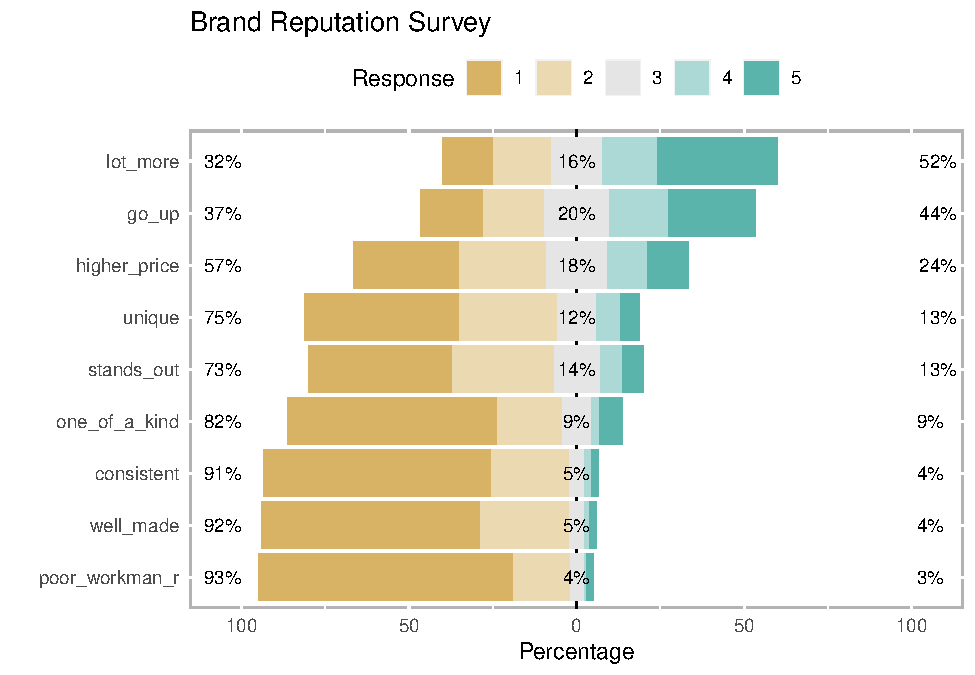
\includegraphics{_main_files/figure-latex/unnamed-chunk-11-1.pdf}

Missing values may mean respondents did not understand the question or did not want to reveal their answer. If \textless5\% of survey responses have no missing values, you can just drop those responses. If missing values are a problem, try the \texttt{Hmisc::naclus()} to see which items tend to be missing in the same record. This survey is clean.

\begin{Shaded}
\begin{Highlighting}[]
\FunctionTok{nrow}\NormalTok{(brand\_rep) }\SpecialCharTok{{-}} \FunctionTok{nrow}\NormalTok{(}\FunctionTok{na.omit}\NormalTok{(brand\_rep)) }\CommentTok{\# num cases}
\DocumentationTok{\#\# [1] 0}
\FunctionTok{colSums}\NormalTok{(}\FunctionTok{is.na}\NormalTok{(brand\_rep)) }\CommentTok{\# num cases by col}
\DocumentationTok{\#\#      well\_made     consistent poor\_workman\_r   higher\_price       lot\_more }
\DocumentationTok{\#\#              0              0              0              0              0 }
\DocumentationTok{\#\#          go\_up     stands\_out         unique  one\_of\_a\_kind }
\DocumentationTok{\#\#              0              0              0              0}
\end{Highlighting}
\end{Shaded}

\hypertarget{correlations}{%
\subsection{Correlations}\label{correlations}}

You will want to identify items that correlate highly with each other, but not highly outside their group. These patterns are the basis of mapping factors to the latent variables. Factors are the concrete survey items; latent variables are the abstract concepts they are intended to supply, like \emph{brand loyalty} or \emph{customer satisfaction}. The correlation plot below appears to have 3 groups, plus a stand-alone variable (\texttt{one\_of\_a\_kind}).

\begin{Shaded}
\begin{Highlighting}[]
\CommentTok{\#psych::corr.test(brand\_rep)}
\NormalTok{corrplot}\SpecialCharTok{::}\FunctionTok{corrplot}\NormalTok{(}\FunctionTok{cor}\NormalTok{(brand\_rep), }\AttributeTok{method =} \StringTok{"circle"}\NormalTok{)}
\end{Highlighting}
\end{Shaded}

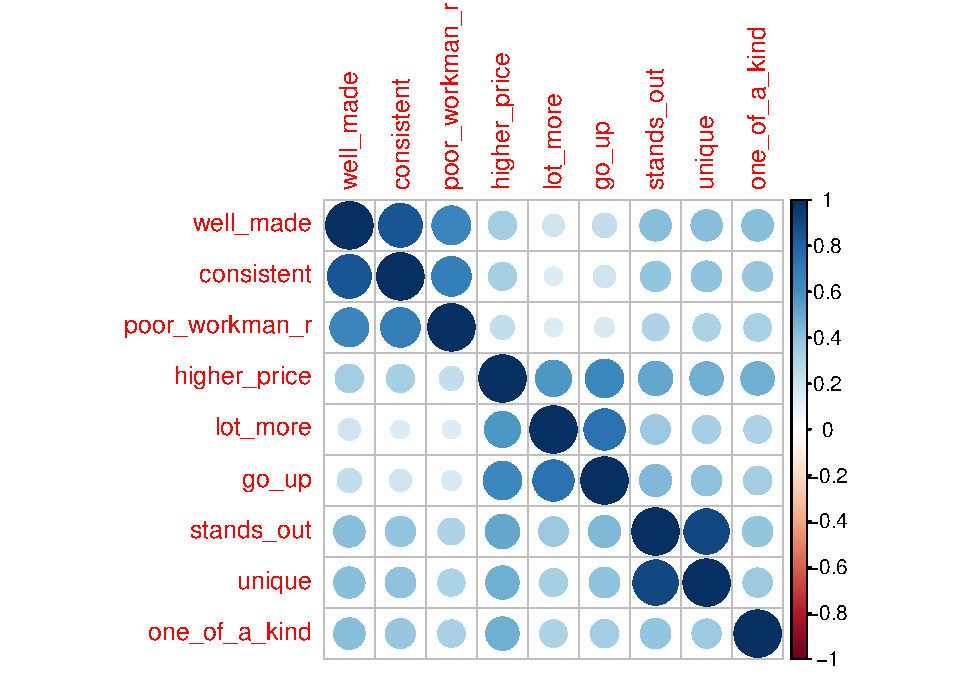
\includegraphics{_main_files/figure-latex/unnamed-chunk-13-1.pdf}

\hypertarget{item-reduction}{%
\section{3. Item Reduction}\label{item-reduction}}

The third phase, explores the mapping of the factors (aka ``manifest variables'') to the latent variable's ``dimensions'' and refines the survey to exclude factors that do not map to a dimension. A latent variable may have several dimensions. E.g., ``brand loyalty'' may consist of ``brand identification'', ``perceived value'', and ``brand trust''. Exploratory factor analysis (EFA), identifies the dimensions in the data, and whether any items do \emph{not} reveal information about the latent variable. EFA establishes the \emph{internal reliability}, whether similar items produce similar scores.

Start with a parallel analysis and scree plot. This will suggest the number of factors in the data. Use this number as the input to an exploratory factor analysis.

\hypertarget{parallel-analysis}{%
\subsection{Parallel Analysis}\label{parallel-analysis}}

A \href{https://www.sciencedirect.com/topics/mathematics/scree-plot}{scree plot} is a line plot of the eigenvalues. An eigenvalue is the proportion of variance explained by each factor. Only factors with eigenvalues greater than those from uncorrelated data are useful. You want to find a sharp reduction in the size of the eigenvalues (like a cliff), with the rest of the smaller eigenvalues constituting rubble (scree!). After the eigenvalues drop dramatically in size, additional factors add relatively little to the information already extracted.

Parallel analysis helps to make the interpretation of scree plots more objective. The eigenvalues are plotted along with eigenvalues of simulated variables with population correlations of 0. The number of eigenvalues above the point where the two lines intersect is the suggested number of factors. The rationale for parallel analysis is that useful factors account for more variance than could be expected by chance.

\texttt{psych::fa.parallel()} compares a scree of your data set to a random data set to identify the number of factors. The elbow below here is at 3 factors.

\begin{Shaded}
\begin{Highlighting}[]
\NormalTok{psych}\SpecialCharTok{::}\FunctionTok{fa.parallel}\NormalTok{(brand\_rep)}
\end{Highlighting}
\end{Shaded}

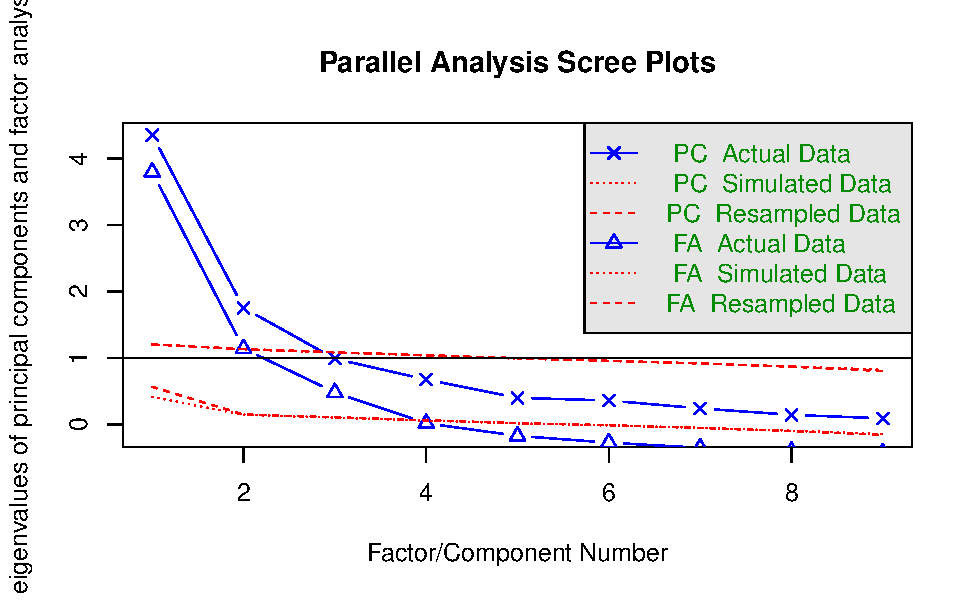
\includegraphics{_main_files/figure-latex/unnamed-chunk-14-1.pdf}

\begin{verbatim}
## Parallel analysis suggests that the number of factors =  3  and the number of components =  2
\end{verbatim}

\hypertarget{exporatory-factor-analysis}{%
\subsection{Exporatory Factor Analysis}\label{exporatory-factor-analysis}}

Use \texttt{psych::fa()} to perform the factor analysis with your chosen number of factors. The number of factors may be the result of your parallel analysis, or the opinion of the SMEs. In this case, we'll go with the 3 factors identified by the parallel analysis.

\begin{Shaded}
\begin{Highlighting}[]
\NormalTok{brand\_rep\_efa }\OtherTok{\textless{}{-}}\NormalTok{ psych}\SpecialCharTok{::}\FunctionTok{fa}\NormalTok{(brand\_rep, }\AttributeTok{nfactors =} \DecValTok{3}\NormalTok{)}
\end{Highlighting}
\end{Shaded}

\begin{verbatim}
## Loading required namespace: GPArotation
\end{verbatim}

\begin{Shaded}
\begin{Highlighting}[]
\CommentTok{\# psych::scree(brand\_rep) \# psych makes scree plot\textquotesingle{}s too.}
\NormalTok{psych}\SpecialCharTok{::}\FunctionTok{fa.diagram}\NormalTok{(brand\_rep\_efa)}
\end{Highlighting}
\end{Shaded}

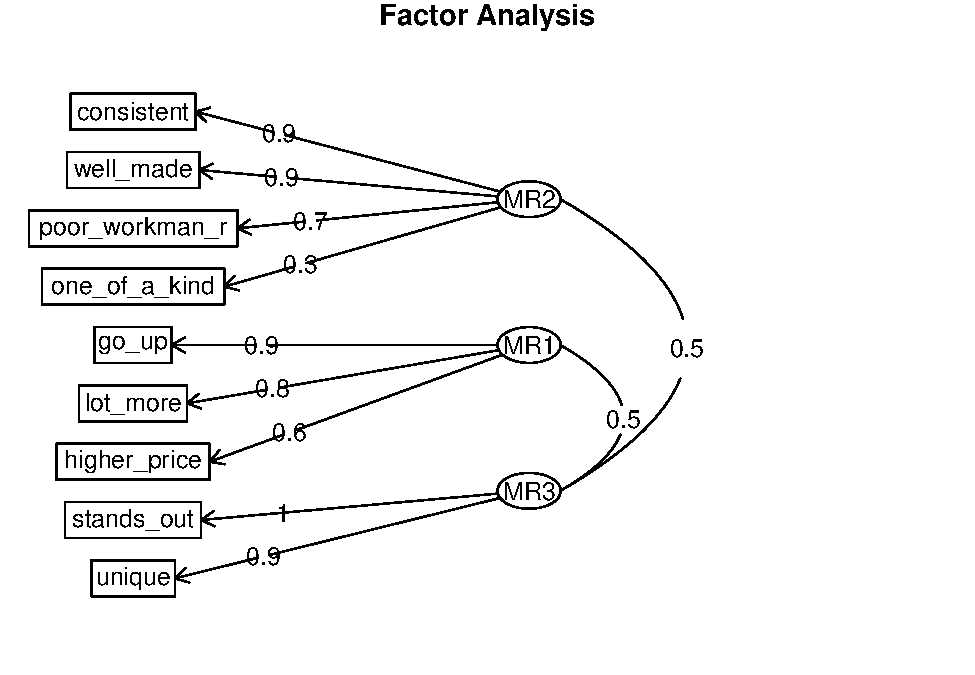
\includegraphics{_main_files/figure-latex/unnamed-chunk-15-1.pdf}

Using EFA, you may tweak the number of factors or drop poorly-loading items. Each item should load highly to one and only one dimension. This one dimension is the item's primary loading. Generally, a primary loading \textgreater{} .7 is excellent, \textgreater.6 is very good, \textgreater.5 is good, \textgreater.4 is fair, and \textless.4 is poor. Here are the factor loadings from the 3 factor model.

\begin{Shaded}
\begin{Highlighting}[]
\NormalTok{brand\_rep\_efa}\SpecialCharTok{$}\NormalTok{loadings}
\end{Highlighting}
\end{Shaded}

\begin{verbatim}
## 
## Loadings:
##                MR2    MR1    MR3   
## well_made       0.896              
## consistent      0.947              
## poor_workman_r  0.739              
## higher_price    0.127  0.632  0.149
## lot_more               0.850       
## go_up                  0.896       
## stands_out                    1.008
## unique                        0.896
## one_of_a_kind   0.309  0.295  0.115
## 
##                  MR2   MR1   MR3
## SS loadings    2.361 2.012 1.858
## Proportion Var 0.262 0.224 0.206
## Cumulative Var 0.262 0.486 0.692
\end{verbatim}

The brand-rep survey items load to 3 factors well except for the \texttt{one\_of\_a\_kind} item. Its primary factor loading (0.309) is poor. The others are either very good (.6-.7) and excellent (\textgreater.7) range.

Look at the model eigenvalues. There should be one eigenvalue per dimension. Eigenvalues a little less than one may be contaminating the model.

\begin{Shaded}
\begin{Highlighting}[]
\NormalTok{brand\_rep\_efa}\SpecialCharTok{$}\NormalTok{e.value}
\end{Highlighting}
\end{Shaded}

\begin{verbatim}
## [1] 4.35629549 1.75381015 0.98701607 0.67377072 0.39901205 0.35865598 0.23915591
## [8] 0.14238807 0.08989556
\end{verbatim}

Look at the factor score correlations. They should all be around 0.6. Much smaller means they are not describing the same latent variable. Much larger means they are describing the same dimension of the latent variable.

\begin{Shaded}
\begin{Highlighting}[]
\NormalTok{brand\_rep\_efa}\SpecialCharTok{$}\NormalTok{r.scores}
\end{Highlighting}
\end{Shaded}

\begin{verbatim}
##           [,1]      [,2]      [,3]
## [1,] 1.0000000 0.3147485 0.4778759
## [2,] 0.3147485 1.0000000 0.5428218
## [3,] 0.4778759 0.5428218 1.0000000
\end{verbatim}

If you have a poorly loaded dimension, drop factors one at a time from the scale. \texttt{one\_of\_a\_kind} loads across all three factors, but does not load strongly onto any one factor. \texttt{one\_of\_a\_kind} is not clearly measuring any dimension of the latent variable. Drop it and try again.

\begin{Shaded}
\begin{Highlighting}[]
\NormalTok{brand\_rep\_efa }\OtherTok{\textless{}{-}}\NormalTok{ psych}\SpecialCharTok{::}\FunctionTok{fa}\NormalTok{(brand\_rep }\SpecialCharTok{\%\textgreater{}\%} \FunctionTok{select}\NormalTok{(}\SpecialCharTok{{-}}\NormalTok{one\_of\_a\_kind), }\AttributeTok{nfactors =} \DecValTok{3}\NormalTok{)}
\NormalTok{brand\_rep\_efa}\SpecialCharTok{$}\NormalTok{loadings}
\end{Highlighting}
\end{Shaded}

\begin{verbatim}
## 
## Loadings:
##                MR2    MR3    MR1   
## well_made       0.887              
## consistent      0.958              
## poor_workman_r  0.735              
## higher_price    0.120  0.596  0.170
## lot_more               0.845       
## go_up                  0.918       
## stands_out                    0.990
## unique                        0.916
## 
##                  MR2   MR3   MR1
## SS loadings    2.261 1.915 1.850
## Proportion Var 0.283 0.239 0.231
## Cumulative Var 0.283 0.522 0.753
\end{verbatim}

\begin{Shaded}
\begin{Highlighting}[]
\NormalTok{brand\_rep\_efa}\SpecialCharTok{$}\NormalTok{e.value}
\end{Highlighting}
\end{Shaded}

\begin{verbatim}
## [1] 4.00884429 1.75380537 0.97785883 0.42232527 0.36214534 0.24086772 0.14404264
## [8] 0.09011054
\end{verbatim}

\begin{Shaded}
\begin{Highlighting}[]
\NormalTok{brand\_rep\_efa}\SpecialCharTok{$}\NormalTok{r.scores}
\end{Highlighting}
\end{Shaded}

\begin{verbatim}
##           [,1]      [,2]      [,3]
## [1,] 1.0000000 0.2978009 0.4802138
## [2,] 0.2978009 1.0000000 0.5351654
## [3,] 0.4802138 0.5351654 1.0000000
\end{verbatim}

This is better. We have three dimensions of brand reputation:

\begin{itemize}
\tightlist
\item
  items \texttt{well\_made}, \texttt{consistent}, and \texttt{poor\_workman\_r} describe \emph{Product Quality},
\item
  items \texttt{higher\_price}, \texttt{lot\_more}, and \texttt{go\_up} describe \emph{Willingness to Pay}, and
\item
  items \texttt{stands\_out} and \texttt{unique} describe \emph{Product Differentiation}
\end{itemize}

Even if the data and your theory suggest otherwise, explore what happens when you include more or fewer factors in your EFA.

\begin{Shaded}
\begin{Highlighting}[]
\NormalTok{psych}\SpecialCharTok{::}\FunctionTok{fa}\NormalTok{(brand\_rep, }\AttributeTok{nfactors =} \DecValTok{2}\NormalTok{)}\SpecialCharTok{$}\NormalTok{loadings}
\end{Highlighting}
\end{Shaded}

\begin{verbatim}
## 
## Loadings:
##                MR1    MR2   
## well_made              0.884
## consistent             0.932
## poor_workman_r         0.728
## higher_price    0.745       
## lot_more        0.784 -0.131
## go_up           0.855 -0.103
## stands_out      0.591  0.286
## unique          0.540  0.307
## one_of_a_kind   0.378  0.305
## 
##                  MR1   MR2
## SS loadings    2.688 2.485
## Proportion Var 0.299 0.276
## Cumulative Var 0.299 0.575
\end{verbatim}

\begin{Shaded}
\begin{Highlighting}[]
\NormalTok{psych}\SpecialCharTok{::}\FunctionTok{fa}\NormalTok{(brand\_rep, }\AttributeTok{nfactors =} \DecValTok{4}\NormalTok{)}\SpecialCharTok{$}\NormalTok{loadings}
\end{Highlighting}
\end{Shaded}

\begin{verbatim}
## 
## Loadings:
##                MR2    MR1    MR3    MR4   
## well_made       0.879                     
## consistent      0.964                     
## poor_workman_r  0.732                     
## higher_price           0.552  0.150  0.168
## lot_more               0.835              
## go_up                  0.929              
## stands_out                    0.976       
## unique                        0.932       
## one_of_a_kind                        0.999
## 
##                  MR2   MR1   MR3   MR4
## SS loadings    2.244 1.866 1.846 1.029
## Proportion Var 0.249 0.207 0.205 0.114
## Cumulative Var 0.249 0.457 0.662 0.776
\end{verbatim}

The two-factor loading worked okay. The 4 factor loading only loaded one variable to the fourth factor. In this example the SME expected a three-factor model and the data did not contradict the theory, so stick with three.

Whereas the item generation phase tested for item equivalence, the EFA phase tests for internal reliability (\emph{consistency}) of items. Internal reliability means the survey produces consistent results. The more common statistics for assessing internal reliability are Cronbach's Alpha, and split-half.

\hypertarget{cronbachs-alpha}{%
\subsection{Cronbach's Alpha}\label{cronbachs-alpha}}

In general, an alpha \textless.6 is unacceptable, \textless.65 is undesirable, \textless.7 is minimally acceptable, \textless.8 is respectable, \textless.9 is very good, and \textgreater=.9 suggests items are \emph{too} alike. A very low alpha means items may not be measuring the same construct, so you should drop items. A very high alpha means items are multicollinear, and you should drop items. Here is Cronbach's alpha for the brand reputation survey, after removing the poorly-loading \texttt{one\_of\_a\_kind} variable.

\begin{Shaded}
\begin{Highlighting}[]
\NormalTok{psych}\SpecialCharTok{::}\FunctionTok{alpha}\NormalTok{(brand\_rep[, }\DecValTok{1}\SpecialCharTok{:}\DecValTok{8}\NormalTok{])}\SpecialCharTok{$}\NormalTok{total}\SpecialCharTok{$}\NormalTok{std.alpha}
\end{Highlighting}
\end{Shaded}

\begin{verbatim}
## [1] 0.8557356
\end{verbatim}

This value is in the ``very good'' range. Cronbach's alpha is often used to measure the reliability of a single dimension. Here are the values for the 3 dimensions.

\begin{Shaded}
\begin{Highlighting}[]
\NormalTok{psych}\SpecialCharTok{::}\FunctionTok{alpha}\NormalTok{(brand\_rep[, }\DecValTok{1}\SpecialCharTok{:}\DecValTok{3}\NormalTok{])}\SpecialCharTok{$}\NormalTok{total}\SpecialCharTok{$}\NormalTok{std }\CommentTok{\# Product Quality}
\DocumentationTok{\#\# [1] 0.8918025}
\NormalTok{psych}\SpecialCharTok{::}\FunctionTok{alpha}\NormalTok{(brand\_rep[, }\DecValTok{4}\SpecialCharTok{:}\DecValTok{6}\NormalTok{])}\SpecialCharTok{$}\NormalTok{total}\SpecialCharTok{$}\NormalTok{std }\CommentTok{\# Willingness to Pay}
\DocumentationTok{\#\# [1] 0.8517566}
\NormalTok{psych}\SpecialCharTok{::}\FunctionTok{alpha}\NormalTok{(brand\_rep[, }\DecValTok{7}\SpecialCharTok{:}\DecValTok{8}\NormalTok{])}\SpecialCharTok{$}\NormalTok{total}\SpecialCharTok{$}\NormalTok{std }\CommentTok{\# Product Differentiation}
\DocumentationTok{\#\# [1] 0.951472}
\end{Highlighting}
\end{Shaded}

Alpha is \textgreater0.7 for each dimension. Sometimes the alpha for our survey as a whole is greater than that of the dimensions. This can happen because Cronbach's alpha is sensitive to the number of items. Over-inflation of the alpha statistic can be a concern when working with surveys containing a large number of items.

\hypertarget{split-half}{%
\subsection{Split-Half}\label{split-half}}

Use \texttt{psych::splitHalf()} to split the survey in half and test whether all parts of the survey contribute equally to measurement. \emph{This method is much less popular than Cronbach's alpha.}

\begin{Shaded}
\begin{Highlighting}[]
\NormalTok{psych}\SpecialCharTok{::}\FunctionTok{splitHalf}\NormalTok{(brand\_rep[, }\DecValTok{1}\SpecialCharTok{:}\DecValTok{8}\NormalTok{])}
\end{Highlighting}
\end{Shaded}

\begin{verbatim}
## Split half reliabilities  
## Call: psych::splitHalf(r = brand_rep[, 1:8])
## 
## Maximum split half reliability (lambda 4) =  0.93
## Guttman lambda 6                          =  0.92
## Average split half reliability            =  0.86
## Guttman lambda 3 (alpha)                  =  0.86
## Guttman lambda 2                          =  0.87
## Minimum split half reliability  (beta)    =  0.66
## Average interitem r =  0.43  with median =  0.4
\end{verbatim}

\hypertarget{confirmatory-factor-analysis}{%
\section{4. Confirmatory Factor Analysis}\label{confirmatory-factor-analysis}}

Whereas EFA is used to develop a theory of the number of factors needed to explain the relationships among the survey items, confirmatory factor analysis (CFA) is a formal hypothesis test of the EFA theory. CFA measures construct validity, that is, whether you are really measuring what you claim to measure.

These notes explain how to use CFA, but do not explain the theory. For that you need to learn about \href{https://www.datacamp.com/courses/dimensionality-reduction-in-r}{dimensionality reduction}, and \href{https://www.datacamp.com/courses/structural-equation-modeling-with-lavaan-in-r}{structural equation modeling}.

Use the \textbf{lavaan} package (latent variable analysis package), passing in the model definition. Here is the model for the three dimensions in the brand reputation survey. Lavaan's default estimator is maximum likelihood, which assumes normality. You can change it to MLR which uses robust standard errors to mitigate non-normality. The summary prints a ton of output. Concentrate on the \texttt{lambda} - the factor loadings.

\begin{Shaded}
\begin{Highlighting}[]
\NormalTok{brand\_rep\_mdl }\OtherTok{\textless{}{-}} \FunctionTok{paste}\NormalTok{(}
  \StringTok{"PrdQl =\textasciitilde{} well\_made + consistent + poor\_workman\_r"}\NormalTok{,}
  \StringTok{"WillPay =\textasciitilde{} higher\_price + lot\_more + go\_up"}\NormalTok{,}
  \StringTok{"PrdDff =\textasciitilde{} stands\_out + unique"}\NormalTok{, }
  \AttributeTok{sep =} \StringTok{"}\SpecialCharTok{\textbackslash{}n}\StringTok{"}
\NormalTok{)}
\NormalTok{brand\_rep\_cfa }\OtherTok{\textless{}{-}}\NormalTok{ lavaan}\SpecialCharTok{::}\FunctionTok{cfa}\NormalTok{(}\AttributeTok{model =}\NormalTok{ brand\_rep\_mdl, }\AttributeTok{data =}\NormalTok{ brand\_rep[, }\DecValTok{1}\SpecialCharTok{:}\DecValTok{8}\NormalTok{], }\AttributeTok{estimator =} \StringTok{"MLR"}\NormalTok{)}
\CommentTok{\# lavaan::summary(brand\_rep\_cfa, fit.measures = TRUE, standardized = TRUE)}
\NormalTok{semPlot}\SpecialCharTok{::}\FunctionTok{semPaths}\NormalTok{(brand\_rep\_cfa, }\AttributeTok{rotation =} \DecValTok{4}\NormalTok{)}
\end{Highlighting}
\end{Shaded}

\begin{verbatim}
## Registered S3 method overwritten by 'kutils':
##   method       from  
##   print.likert likert
\end{verbatim}

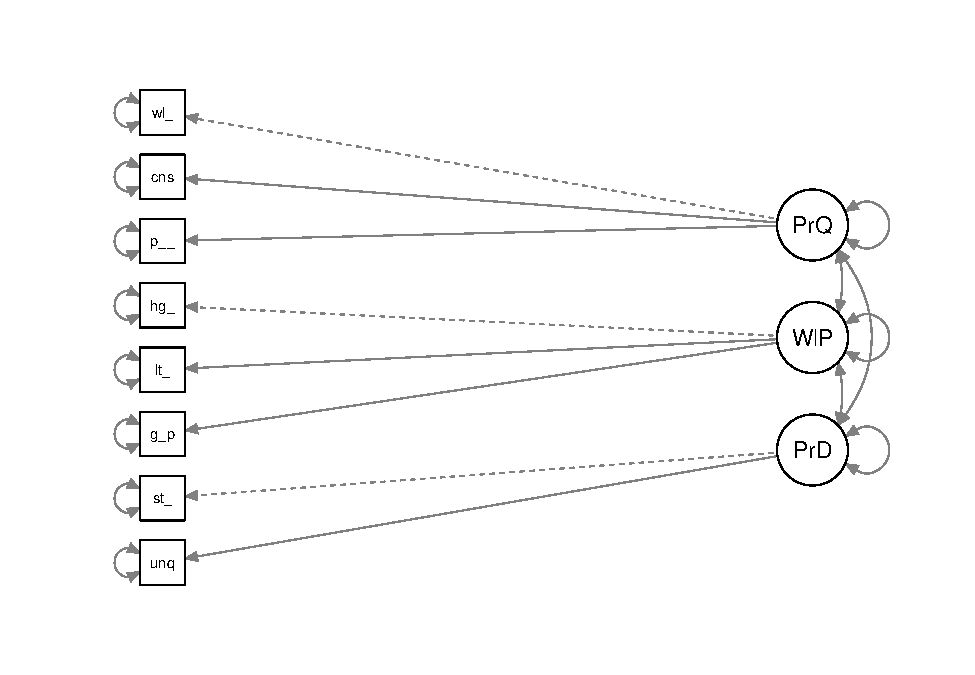
\includegraphics{_main_files/figure-latex/unnamed-chunk-24-1.pdf}

\begin{Shaded}
\begin{Highlighting}[]
\NormalTok{lavaan}\SpecialCharTok{::}\FunctionTok{inspect}\NormalTok{(brand\_rep\_cfa, }\StringTok{"std"}\NormalTok{)}\SpecialCharTok{$}\NormalTok{lambda}
\end{Highlighting}
\end{Shaded}

\begin{verbatim}
##                PrdQl WillPy PrdDff
## well_made      0.914  0.000  0.000
## consistent     0.932  0.000  0.000
## poor_workman_r 0.730  0.000  0.000
## higher_price   0.000  0.733  0.000
## lot_more       0.000  0.812  0.000
## go_up          0.000  0.902  0.000
## stands_out     0.000  0.000  0.976
## unique         0.000  0.000  0.930
\end{verbatim}

The CFA hypothesis test is a chi-square test, so is sensitive to normality assumptions and n-size. Other fit measure are reported too:
* Comparative Fit Index (CFI) (look for value \textgreater.9)
* Tucker-Lewis Index (TLI) (look for value \textgreater.9)
* Root mean squared Error of Approximation (RMSEA) (look for value \textless.05)

There are actually 71 fit measures to choose from! Focus on CFI and TLI.

\begin{Shaded}
\begin{Highlighting}[]
\NormalTok{lavaan}\SpecialCharTok{::}\FunctionTok{fitMeasures}\NormalTok{(brand\_rep\_cfa, }\AttributeTok{fit.measures =} \FunctionTok{c}\NormalTok{(}\StringTok{"cfi"}\NormalTok{, }\StringTok{"tli"}\NormalTok{))}
\end{Highlighting}
\end{Shaded}

\begin{verbatim}
##   cfi   tli 
## 0.980 0.967
\end{verbatim}

This output indicates a good model because both measures are \textgreater.9. Check the standardized estimates for each item. The standardized factor loadings are the basis of establishing construct validity. While we call these measures `loadings,' they are better described as correlations of each manifest item with the dimensions. As you calculated, the difference between a perfect correlation and the observed is considered `error.' This relationship between the so-called `true' and `observed' scores is the basis of classical test theory.

\begin{Shaded}
\begin{Highlighting}[]
\NormalTok{lavaan}\SpecialCharTok{::}\FunctionTok{standardizedSolution}\NormalTok{(brand\_rep\_cfa) }\SpecialCharTok{\%\textgreater{}\%}
  \FunctionTok{filter}\NormalTok{(op }\SpecialCharTok{==} \StringTok{"=\textasciitilde{}"}\NormalTok{) }\SpecialCharTok{\%\textgreater{}\%}
  \FunctionTok{select}\NormalTok{(lhs, rhs, est.std, pvalue)}
\end{Highlighting}
\end{Shaded}

\begin{verbatim}
##       lhs            rhs est.std pvalue
## 1   PrdQl      well_made   0.914      0
## 2   PrdQl     consistent   0.932      0
## 3   PrdQl poor_workman_r   0.730      0
## 4 WillPay   higher_price   0.733      0
## 5 WillPay       lot_more   0.812      0
## 6 WillPay          go_up   0.902      0
## 7  PrdDff     stands_out   0.976      0
## 8  PrdDff         unique   0.930      0
\end{verbatim}

If you have a survey that meets your assumptions, performs well under EFA, but fails under CFA, return to your survey and revisit your scale, examine the CFA modification indices, factor variances, etc.

\hypertarget{convergentdiscriminant-validity}{%
\section{5. Convergent/Discriminant Validity}\label{convergentdiscriminant-validity}}

Construct validity means the survey measures what it intends to measure. It is composed of convergent validity and discriminant validity. Convergent validity means factors address the same concept. Discriminant validity means factors address different aspects of the concept.

Test for construct validity \emph{after} assessing CFA model strength (with CFI, TFI, and RMSEA) -- a poor-fitting model may have greater construct validity than a better-fitting model. Use the \texttt{semTools::reliability()} function. The average variance extracted (AVE) measures convergent validity (\texttt{avevar}) and should be \textgreater{} .5. The composite reliability (CR) measures discriminant validity (\texttt{omega}) and should be \textgreater{} .7.

\begin{Shaded}
\begin{Highlighting}[]
\NormalTok{semTools}\SpecialCharTok{::}\FunctionTok{reliability}\NormalTok{(brand\_rep\_cfa)}
\end{Highlighting}
\end{Shaded}

\begin{verbatim}
##            PrdQl   WillPay    PrdDff
## alpha  0.8926349 0.8521873 0.9514719
## omega  0.9017514 0.8605751 0.9520117
## omega2 0.9017514 0.8605751 0.9520117
## omega3 0.9019287 0.8646975 0.9520114
## avevar 0.7573092 0.6756174 0.9084654
\end{verbatim}

These values look good for all three dimensions. As an aside, \texttt{alpha} is Cronbach's alpha. Do not be tempted to test reliability and validity in the same step. Start with reliability because it is a necessary but insufficient condition for validity. By checking for internal consistency first, as measured by alpha, then construct validity, as measured by AVE and CR, you establish the necessary reliability of the scale as a whole was met, then took it to the next level by checking for construct validity among the unique dimensions.

At this point you have established that the latent and manifest variables are related as hypothesized, and that the survey measures what you intended to measure, in this case, brand reputation.

\hypertarget{replication}{%
\section{6. Replication}\label{replication}}

The replication phase establishes criterion validity and stability (reliability). Criterion validity is a measure of the relationship between the construct and some external measure of interest. Measure criterion validity with \emph{concurrent validity}, how well items correlate with an external metric measured at the same time, and with \emph{predictive validity}, how well an item predicts an external metric. Stability means the survey produces similar results over repeated \emph{test-retest} administrations.

\hypertarget{criterion-validity}{%
\subsection{Criterion Validity}\label{criterion-validity}}

\hypertarget{concurrent-validity}{%
\subsubsection{Concurrent Validity}\label{concurrent-validity}}

Concurrent validity is a measure of whether our latent construct is significantly correlated to some outcome measured at the same time.

Suppose you have an additional data set of consumer spending on the brand. The consumer's perception of the brand should correlate with their spending. Before checking for concurrent validity, standardize the data so that likert and other variable types are on the same scale.

\begin{Shaded}
\begin{Highlighting}[]
\FunctionTok{set.seed}\NormalTok{(}\DecValTok{20201004}\NormalTok{)}
\NormalTok{brand\_rep }\OtherTok{\textless{}{-}}\NormalTok{ brand\_rep }\SpecialCharTok{\%\textgreater{}\%}
  \FunctionTok{mutate}\NormalTok{(}\AttributeTok{spend =}\NormalTok{ ((well\_made }\SpecialCharTok{+}\NormalTok{ consistent }\SpecialCharTok{+}\NormalTok{ poor\_workman\_r)}\SpecialCharTok{/}\DecValTok{3} \SpecialCharTok{*} \DecValTok{5} \SpecialCharTok{+}
\NormalTok{                  (higher\_price }\SpecialCharTok{+}\NormalTok{ lot\_more }\SpecialCharTok{+}\NormalTok{ go\_up)}\SpecialCharTok{/}\DecValTok{3} \SpecialCharTok{*} \DecValTok{3} \SpecialCharTok{+}
\NormalTok{                  (stands\_out }\SpecialCharTok{+}\NormalTok{ unique)}\SpecialCharTok{/}\DecValTok{2} \SpecialCharTok{*} \DecValTok{2}\NormalTok{) }\SpecialCharTok{/} \DecValTok{10}\NormalTok{)}
\NormalTok{brand\_rep}\SpecialCharTok{$}\NormalTok{spend }\OtherTok{\textless{}{-}}\NormalTok{ brand\_rep}\SpecialCharTok{$}\NormalTok{spend }\SpecialCharTok{+} \FunctionTok{rnorm}\NormalTok{(}\DecValTok{559}\NormalTok{, }\DecValTok{5}\NormalTok{, }\DecValTok{4}\NormalTok{) }\CommentTok{\# add randomness}
\NormalTok{brand\_rep\_scaled }\OtherTok{\textless{}{-}} \FunctionTok{scale}\NormalTok{(brand\_rep)}
\end{Highlighting}
\end{Shaded}

Do respondents with higher scores on our the brand reputation scale also tend to spend more at the store? Build model, and latentize \texttt{spend} as \texttt{Spndng} and model with the \texttt{\textasciitilde{}\textasciitilde{}} operator. Fit the model with the \texttt{semTools::sem()} function.

\begin{Shaded}
\begin{Highlighting}[]
\NormalTok{brand\_rep\_cv\_mdl }\OtherTok{\textless{}{-}} \FunctionTok{paste}\NormalTok{(}
  \StringTok{"PrdQl =\textasciitilde{} well\_made + consistent + poor\_workman\_r"}\NormalTok{,}
  \StringTok{"WillPay =\textasciitilde{} higher\_price + lot\_more + go\_up"}\NormalTok{,}
  \StringTok{"PrdDff =\textasciitilde{} stands\_out + unique"}\NormalTok{,}
  \StringTok{"Spndng =\textasciitilde{} spend"}\NormalTok{,}
  \StringTok{"Spndng \textasciitilde{}\textasciitilde{} PrdQl + WillPay + PrdDff"}\NormalTok{,}
  \AttributeTok{sep =} \StringTok{"}\SpecialCharTok{\textbackslash{}n}\StringTok{"}
\NormalTok{)}
\NormalTok{brand\_rep\_cv }\OtherTok{\textless{}{-}}\NormalTok{ lavaan}\SpecialCharTok{::}\FunctionTok{sem}\NormalTok{(}\AttributeTok{data =}\NormalTok{ brand\_rep\_scaled, }\AttributeTok{model =}\NormalTok{ brand\_rep\_cv\_mdl)}
\end{Highlighting}
\end{Shaded}

Here are the standardized covariances. Because the data is standardized, interpret these as correlations. The p-vales are not significant because the spending data was random.

\begin{Shaded}
\begin{Highlighting}[]
\NormalTok{lavaan}\SpecialCharTok{::}\FunctionTok{standardizedSolution}\NormalTok{(brand\_rep\_cv) }\SpecialCharTok{\%\textgreater{}\%} 
  \FunctionTok{filter}\NormalTok{(rhs }\SpecialCharTok{==} \StringTok{"Spndng"}\NormalTok{) }\SpecialCharTok{\%\textgreater{}\%}
  \FunctionTok{select}\NormalTok{(}\SpecialCharTok{{-}}\NormalTok{op, }\SpecialCharTok{{-}}\NormalTok{rhs)}
\end{Highlighting}
\end{Shaded}

\begin{verbatim}
##       lhs est.std    se     z pvalue ci.lower ci.upper
## 1   PrdQl   0.174 0.043 4.092      0    0.091    0.258
## 2 WillPay   0.241 0.043 5.654      0    0.157    0.324
## 3  PrdDff   0.198 0.041 4.779      0    0.117    0.279
## 4  Spndng   1.000 0.000    NA     NA    1.000    1.000
\end{verbatim}

\begin{Shaded}
\begin{Highlighting}[]
\NormalTok{semPlot}\SpecialCharTok{::}\FunctionTok{semPaths}\NormalTok{(brand\_rep\_cv, }\AttributeTok{whatLabels =} \StringTok{"est.std"}\NormalTok{, }\AttributeTok{edge.label.cex =}\NormalTok{ .}\DecValTok{8}\NormalTok{, }\AttributeTok{rotation =} \DecValTok{2}\NormalTok{)}
\end{Highlighting}
\end{Shaded}

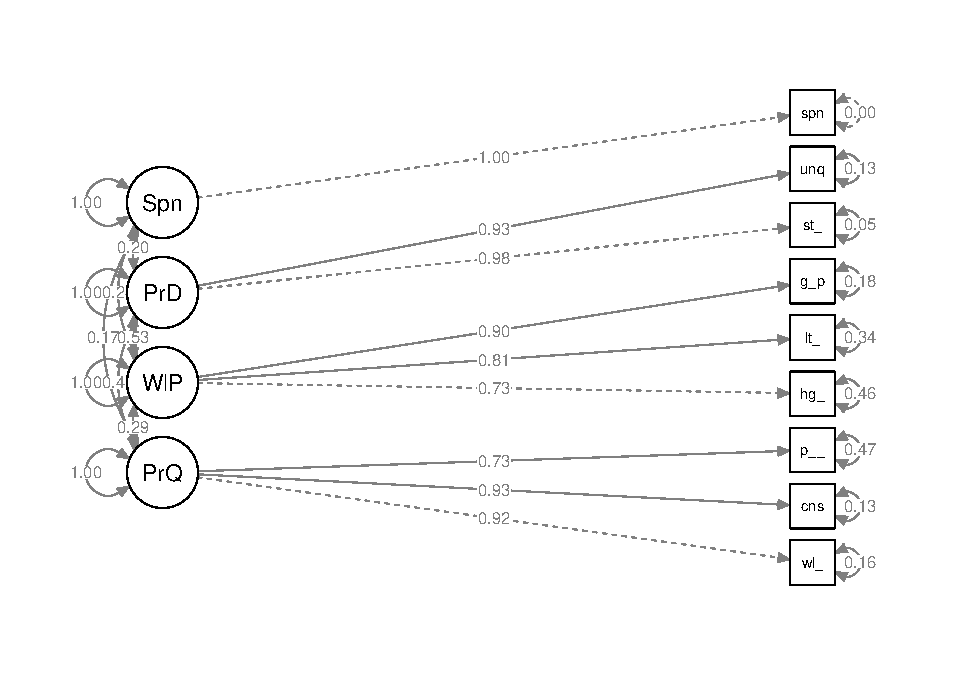
\includegraphics{_main_files/figure-latex/unnamed-chunk-30-1.pdf}

Each dimension of brand reputation is positively correlated to spending history and the relationships are all significant.

\hypertarget{predictive-validity}{%
\subsubsection{Predictive Validity}\label{predictive-validity}}

Predictive validity is established by regressing some future outcome on your established construct. Assess predictive validity just as you would with any linear regression -- regression estimates and p-values (\texttt{starndardizedSolution()}), and the r-squared coefficient of determination \texttt{inspect()}.

Build a regression model with the single \texttt{\textasciitilde{}} operator. Then fit the model to the data as before.

\begin{Shaded}
\begin{Highlighting}[]
\NormalTok{brand\_rep\_pv\_mdl }\OtherTok{\textless{}{-}} \FunctionTok{paste}\NormalTok{(}
  \StringTok{"PrdQl =\textasciitilde{} well\_made + consistent + poor\_workman\_r"}\NormalTok{,}
  \StringTok{"WillPay =\textasciitilde{} higher\_price + lot\_more + go\_up"}\NormalTok{,}
  \StringTok{"PrdDff =\textasciitilde{} stands\_out + unique"}\NormalTok{,}
  \StringTok{"spend \textasciitilde{} PrdQl + WillPay + PrdDff"}\NormalTok{,}
  \AttributeTok{sep =} \StringTok{"}\SpecialCharTok{\textbackslash{}n}\StringTok{"}
\NormalTok{)}
\NormalTok{brand\_rep\_pv }\OtherTok{\textless{}{-}}\NormalTok{ lavaan}\SpecialCharTok{::}\FunctionTok{sem}\NormalTok{(}\AttributeTok{data =}\NormalTok{ brand\_rep\_scaled, }\AttributeTok{model =}\NormalTok{ brand\_rep\_pv\_mdl)}
\CommentTok{\#lavaan::summary(brand\_rep\_pv, standardized = T, fit.measures = T, rsquare = T)}
\NormalTok{semPlot}\SpecialCharTok{::}\FunctionTok{semPaths}\NormalTok{(brand\_rep\_pv, }\AttributeTok{whatLabels =} \StringTok{"est.std"}\NormalTok{, }\AttributeTok{edge.label.cex =}\NormalTok{ .}\DecValTok{8}\NormalTok{, }\AttributeTok{rotation =} \DecValTok{2}\NormalTok{)}
\end{Highlighting}
\end{Shaded}

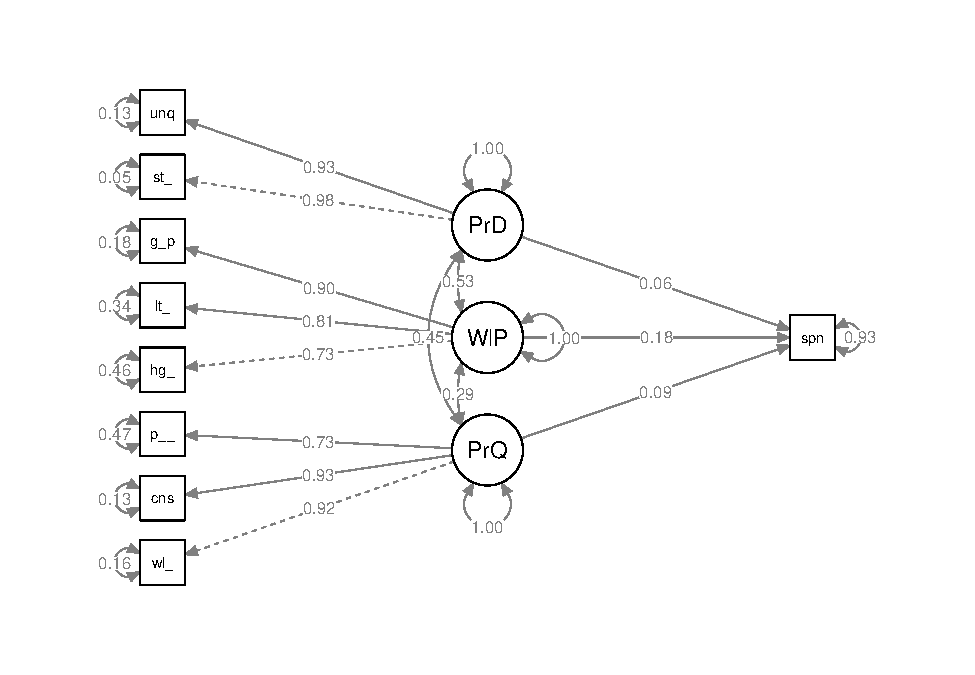
\includegraphics{_main_files/figure-latex/unnamed-chunk-31-1.pdf}

\begin{Shaded}
\begin{Highlighting}[]
\NormalTok{lavaan}\SpecialCharTok{::}\FunctionTok{standardizedSolution}\NormalTok{(brand\_rep\_pv) }\SpecialCharTok{\%\textgreater{}\%} 
  \FunctionTok{filter}\NormalTok{(op }\SpecialCharTok{==} \StringTok{"\textasciitilde{}"}\NormalTok{) }\SpecialCharTok{\%\textgreater{}\%}
  \FunctionTok{mutate\_if}\NormalTok{(is.numeric, round, }\AttributeTok{digits =} \DecValTok{3}\NormalTok{)}
\end{Highlighting}
\end{Shaded}

\begin{verbatim}
##     lhs op     rhs est.std    se     z pvalue ci.lower ci.upper
## 1 spend  ~   PrdQl   0.094 0.048 1.949  0.051   -0.001    0.189
## 2 spend  ~ WillPay   0.182 0.052 3.486  0.000    0.080    0.284
## 3 spend  ~  PrdDff   0.060 0.055 1.092  0.275   -0.047    0.167
\end{verbatim}

\begin{Shaded}
\begin{Highlighting}[]
\NormalTok{lavaan}\SpecialCharTok{::}\FunctionTok{inspect}\NormalTok{(brand\_rep\_pv, }\StringTok{"r2"}\NormalTok{)}
\end{Highlighting}
\end{Shaded}

\begin{verbatim}
##      well_made     consistent poor_workman_r   higher_price       lot_more 
##          0.837          0.867          0.533          0.537          0.658 
##          go_up     stands_out         unique          spend 
##          0.816          0.951          0.866          0.072
\end{verbatim}

There is a statistically significant relationship between one dimension of brand quality (Willingness to Pay) and spending. At this point you may want to drop the other two dimensions. However, the R\^{}2 is not good - only 7\% of the variability in Spending can be explained by the three dimension of our construct.

Factor scores represent individual respondents' standing on a latent factor. While not used for scale validation per se, factor scores can be used for customer segmentation via clustering, network analysis and other statistical techniques.

\begin{Shaded}
\begin{Highlighting}[]
\NormalTok{brand\_rep\_cfa }\OtherTok{\textless{}{-}}\NormalTok{ lavaan}\SpecialCharTok{::}\FunctionTok{cfa}\NormalTok{(brand\_rep\_pv\_mdl, }\AttributeTok{data =}\NormalTok{ brand\_rep\_scaled)}

\NormalTok{brand\_rep\_cfa\_scores }\OtherTok{\textless{}{-}}\NormalTok{ lavaan}\SpecialCharTok{::}\FunctionTok{predict}\NormalTok{(brand\_rep\_cfa) }\SpecialCharTok{\%\textgreater{}\%} \FunctionTok{as.data.frame}\NormalTok{()}
\NormalTok{psych}\SpecialCharTok{::}\FunctionTok{describe}\NormalTok{(brand\_rep\_cfa\_scores)}
\end{Highlighting}
\end{Shaded}

\begin{verbatim}
##         vars   n mean   sd median trimmed  mad   min  max range  skew kurtosis
## PrdQl      1 559    0 0.88  -0.50   -0.19 0.09 -0.57 4.02  4.59  2.31     6.18
## WillPay    2 559    0 0.69   0.00    0.01 0.86 -1.15 1.16  2.31 -0.05    -1.18
## PrdDff     3 559    0 0.96  -0.04   -0.15 1.17 -0.88 2.54  3.41  1.09     0.35
##           se
## PrdQl   0.04
## WillPay 0.03
## PrdDff  0.04
\end{verbatim}

\begin{Shaded}
\begin{Highlighting}[]
\NormalTok{psych}\SpecialCharTok{::}\FunctionTok{multi.hist}\NormalTok{(brand\_rep\_cfa\_scores)}
\end{Highlighting}
\end{Shaded}

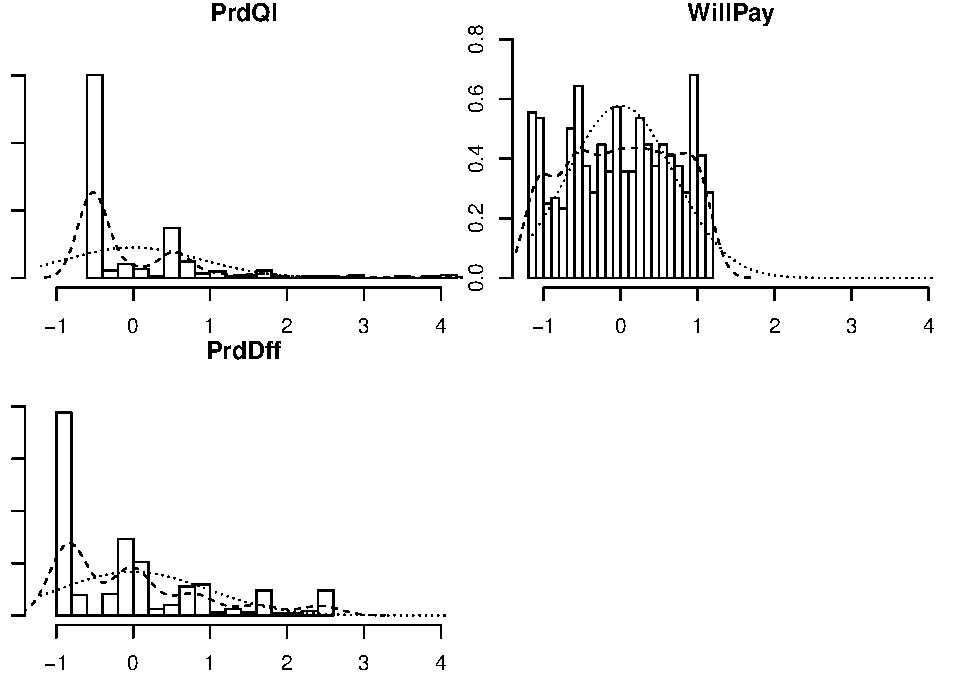
\includegraphics{_main_files/figure-latex/test385-1.pdf}

\begin{Shaded}
\begin{Highlighting}[]
\FunctionTok{map}\NormalTok{(brand\_rep\_cfa\_scores, shapiro.test)}
\end{Highlighting}
\end{Shaded}

\begin{verbatim}
## $PrdQl
## 
##  Shapiro-Wilk normality test
## 
## data:  .x[[i]]
## W = 0.66986, p-value < 2.2e-16
## 
## 
## $WillPay
## 
##  Shapiro-Wilk normality test
## 
## data:  .x[[i]]
## W = 0.94986, p-value = 7.811e-13
## 
## 
## $PrdDff
## 
##  Shapiro-Wilk normality test
## 
## data:  .x[[i]]
## W = 0.82818, p-value < 2.2e-16
\end{verbatim}

These scores are not normally distributed, which makes clustering a great choice for modeling factor scores. Clustering does not mean distance-based clustering, such as K-means, in this context. Mixture models consider data as coming from a distribution which itself is a mixture of clusters. To learn more about model-based clustering in the \href{https://www.datacamp.com/courses/hierarchical-and-mixed-effects-models}{Hierarchical and Mixed Effects Models} DataCamp course.

Factor scores can be extracted from a structural equation model and used as inputs in other models. For example, you can use the factor scores from the brand reputation dimensions as regressors for a regrssion on spending.

\begin{Shaded}
\begin{Highlighting}[]
\NormalTok{brand\_rep\_fs\_reg\_dat }\OtherTok{\textless{}{-}} \FunctionTok{bind\_cols}\NormalTok{(brand\_rep\_cfa\_scores, }\AttributeTok{spend =}\NormalTok{ brand\_rep}\SpecialCharTok{$}\NormalTok{spend)}
\NormalTok{brand\_rep\_fs\_reg }\OtherTok{\textless{}{-}} \FunctionTok{lm}\NormalTok{(spend }\SpecialCharTok{\textasciitilde{}}\NormalTok{ PrdQl }\SpecialCharTok{+}\NormalTok{ WillPay }\SpecialCharTok{+}\NormalTok{ PrdDff, }\AttributeTok{data =}\NormalTok{ brand\_rep\_fs\_reg\_dat)}
\FunctionTok{summary}\NormalTok{(brand\_rep\_fs\_reg)}\SpecialCharTok{$}\NormalTok{coef}
\end{Highlighting}
\end{Shaded}

\begin{verbatim}
##              Estimate Std. Error    t value      Pr(>|t|)
## (Intercept) 7.1555354  0.1591195 44.9695738 3.363705e-187
## PrdQl       0.4260875  0.2062002  2.0663774  3.925620e-02
## WillPay     1.1365087  0.2805960  4.0503388  5.842799e-05
## PrdDff      0.1714031  0.2181813  0.7855993  4.324375e-01
\end{verbatim}

The coefficients and r-squared of the lm() and sem() models closely resemble each other, but keeping the regression inside the lavaan framework provides more information (as witnessed in the higher estimates and r-squared). A construct, once validated, can be combined with a wide range of outcomes and models to produce valuable information about consumer behavior and habits.

\hypertarget{test-retest-reliability}{%
\subsection{Test-Retest Reliability}\label{test-retest-reliability}}

Test-retest reliability is the ability to achieve the same result from a respondent at two closely-spaced points in time (repeated measures).

Suppose you had two surveys, identified by an \texttt{id} field.

\begin{Shaded}
\begin{Highlighting}[]
\CommentTok{\# svy\_1 \textless{}{-} brand\_rep[sample(1:559, 300),] \%\textgreater{}\% as.data.frame()}
\CommentTok{\# svy\_2 \textless{}{-} brand\_rep[sample(1:559, 300),] \%\textgreater{}\% as.data.frame()}
\CommentTok{\# survey\_test\_retest \textless{}{-} psych::testRetest(t1 = svy\_1, t2 = svy\_2, id = "id")}
\CommentTok{\# survey\_test\_retest$r12}
\end{Highlighting}
\end{Shaded}

An r\^{}2 \textless.7 is unacceptable, \textless.9 good, and \textgreater.9 very good. This one is unacceptable.

One way to check for replication is by splitting the data in half.

\begin{Shaded}
\begin{Highlighting}[]
\CommentTok{\# svy \textless{}{-} bind\_rows(svy\_1, svy\_2, .id = "time")}
\CommentTok{\# }
\CommentTok{\# psych::describeBy(svy, "time")}
\CommentTok{\# }
\CommentTok{\# brand\_rep\_test\_retest \textless{}{-} psych::testRetest(}
\CommentTok{\#   t1 = filter(svy, time == 1),}
\CommentTok{\#   t2 = filter(svy, time == 2),}
\CommentTok{\#   id = "id")}
\CommentTok{\# }
\CommentTok{\# brand\_rep\_test\_retest$r12}
\end{Highlighting}
\end{Shaded}

If the correlation of scaled scores across time 1 and time 2 is greater than .9, that indicates very strong test-retest reliability. This measure can be difficult to collect because it requires the same respondents to answer the survey at two points in time. However, it's a good technique to have in your survey development toolkit.

When validating a scale, it's a good idea to split the survey results into two samples, using one for EFA and one for CFA. This works as a sort of cross-validation such that the overall fit of the model is less likely due to chance of any one sample's makeup.

\begin{Shaded}
\begin{Highlighting}[]
\CommentTok{\# brand\_rep\_efa\_data \textless{}{-} brand\_rep[1:280,]}
\CommentTok{\# brand\_rep\_cfa\_data \textless{}{-} brand\_rep[281:559,]}
\CommentTok{\#  }
\CommentTok{\# efa \textless{}{-} psych::fa(brand\_rep\_efa\_data, nfactors = 3)}
\CommentTok{\# efa$loadings}
\CommentTok{\# }
\CommentTok{\# brand\_rep\_cfa \textless{}{-} lavaan::cfa(brand\_rep\_mdl, data = brand\_rep\_cfa\_data)}
\CommentTok{\# lavaan::inspect(brand\_rep\_cfa, what = "call")}
\CommentTok{\# }
\CommentTok{\# lavaan::fitmeasures(brand\_rep\_cfa)[c("cfi","tli","rmsea")]}
\end{Highlighting}
\end{Shaded}

\hypertarget{analyzing-survey-data}{%
\chapter{Analyzing Survey Data}\label{analyzing-survey-data}}

This is a tutorial for using the \textbf{survey} package \citep{R-survey} to analyze complex survey data. ``Complex'' surveys are those with stratification and/or clustering. The package handles weights, and adjusts statistical tests for the survey design.

\hypertarget{defining-the-survey-design}{%
\section{Defining the Survey Design}\label{defining-the-survey-design}}

Below are some examples defining the most common survey designs. The \textbf{survey} package includes the \emph{Student performance in California schools} data set (\texttt{api}), a record of the Academic Performance Index based on standardized testing. \texttt{api} contains sub-data sets that illustrate the design types.

\begin{itemize}
\tightlist
\item
  \texttt{apisrs} is a simple random sample of (\emph{n} = 200) schools,
\item
  \texttt{apistrat} is stratified sample of 3 school types (elementary, middle, high) with simple random sampling of different sizes in each stratum,
\item
  \texttt{apiclus2} is a two-stage cluster sample of schools within districts.
\end{itemize}

You create a survey design object with the \texttt{svydesign(data,\ ...)} function. There are parameter settings for each design type.

\hypertarget{simple-random-sample}{%
\subsection{Simple Random Sample}\label{simple-random-sample}}

A simple random sample has no clusters, so indicate this with \texttt{ids\ =\ \textasciitilde{}1}. The response weights will always be the same, equaling the population size divided by the sample size. Typically, the response weight is identified in a column. There is another parameter called the finite population correction (\texttt{fpc}) that is used to reduce the variance when a substantial fraction of the total population has been sampled. Set \texttt{fpc} to the stratum population size. A simple random sample has no strata, so it will always be the same, equaling the population size.

For \texttt{apisrs} the population size is 6,194 (the number of schools in California). The sample size is 200, so the response weights all equal 6,194 / 200 = 30.97.

\begin{Shaded}
\begin{Highlighting}[]
\FunctionTok{nrow}\NormalTok{(apisrs)}
\DocumentationTok{\#\# [1] 200}
\NormalTok{apisrs }\SpecialCharTok{\%\textgreater{}\%} \FunctionTok{count}\NormalTok{(pw, fpc)}
\DocumentationTok{\#\#      pw  fpc   n}
\DocumentationTok{\#\# 1 30.97 6194 200}
\end{Highlighting}
\end{Shaded}

Here is the design object.

\begin{Shaded}
\begin{Highlighting}[]
\NormalTok{apisrs\_design }\OtherTok{\textless{}{-}} \FunctionTok{svydesign}\NormalTok{(}
  \AttributeTok{data =}\NormalTok{ apisrs, }
  \AttributeTok{weights =} \SpecialCharTok{\textasciitilde{}}\NormalTok{pw, }
  \AttributeTok{fpc =} \SpecialCharTok{\textasciitilde{}}\NormalTok{fpc, }
  \AttributeTok{ids =} \SpecialCharTok{\textasciitilde{}}\DecValTok{1}
\NormalTok{)}
\FunctionTok{summary}\NormalTok{(apisrs\_design)}
\DocumentationTok{\#\# Independent Sampling design}
\DocumentationTok{\#\# svydesign(data = apisrs, weights = \textasciitilde{}pw, fpc = \textasciitilde{}fpc, ids = \textasciitilde{}1)}
\DocumentationTok{\#\# Probabilities:}
\DocumentationTok{\#\#    Min. 1st Qu.  Median    Mean 3rd Qu.    Max. }
\DocumentationTok{\#\# 0.03229 0.03229 0.03229 0.03229 0.03229 0.03229 }
\DocumentationTok{\#\# Population size (PSUs): 6194 }
\DocumentationTok{\#\# Data variables:}
\DocumentationTok{\#\#  [1] "cds"      "stype"    "name"     "sname"    "snum"     "dname"   }
\DocumentationTok{\#\#  [7] "dnum"     "cname"    "cnum"     "flag"     "pcttest"  "api00"   }
\DocumentationTok{\#\# [13] "api99"    "target"   "growth"   "sch.wide" "comp.imp" "both"    }
\DocumentationTok{\#\# [19] "awards"   "meals"    "ell"      "yr.rnd"   "mobility" "acs.k3"  }
\DocumentationTok{\#\# [25] "acs.46"   "acs.core" "pct.resp" "not.hsg"  "hsg"      "some.col"}
\DocumentationTok{\#\# [31] "col.grad" "grad.sch" "avg.ed"   "full"     "emer"     "enroll"  }
\DocumentationTok{\#\# [37] "api.stu"  "pw"       "fpc"}
\end{Highlighting}
\end{Shaded}

\hypertarget{stratified-sample}{%
\subsection{Stratified Sample}\label{stratified-sample}}

Define a stratified sample by specifying with the \texttt{strata} parameter. The schools in \texttt{apistrat} are stratified based on the school type \emph{E} = Elementary, \emph{M} = Middle, and \emph{H} = High School. For each school type, a simple random sample of schools was taken: \(n_E\) = 100, \(n_M\) = 50, and \(n_H\) = 50. The 100 elementary schools represent 100 / 4,421 of the state's elementary schools, so their weights = 44.21. Similarly, the weights are 50 / 1,018 = 20.36 for the middle schools, and 50 / 755 = 15.10 for the high schools.

\begin{Shaded}
\begin{Highlighting}[]
\NormalTok{apistrat }\SpecialCharTok{\%\textgreater{}\%} 
  \FunctionTok{count}\NormalTok{(stype, pw, fpc) }\SpecialCharTok{\%\textgreater{}\%} 
  \FunctionTok{mutate}\NormalTok{(}\StringTok{\textasciigrave{}}\AttributeTok{pw*n}\StringTok{\textasciigrave{}} \OtherTok{=}\NormalTok{ pw }\SpecialCharTok{*}\NormalTok{ n) }\SpecialCharTok{\%\textgreater{}\%}
  \FunctionTok{adorn\_totals}\NormalTok{(,,,, }\SpecialCharTok{{-}}\NormalTok{pw) }\SpecialCharTok{\%\textgreater{}\%} 
  \FunctionTok{flextable}\NormalTok{() }\SpecialCharTok{\%\textgreater{}\%} \FunctionTok{colformat\_num}\NormalTok{(}\AttributeTok{j =} \DecValTok{2}\NormalTok{, }\AttributeTok{digits =} \DecValTok{2}\NormalTok{) }\SpecialCharTok{\%\textgreater{}\%} \FunctionTok{colformat\_int}\NormalTok{(}\AttributeTok{j =} \FunctionTok{c}\NormalTok{(}\DecValTok{3}\SpecialCharTok{:}\DecValTok{5}\NormalTok{))}
\end{Highlighting}
\end{Shaded}

\providecommand{\docline}[3]{\noalign{\global\setlength{\arrayrulewidth}{#1}}\arrayrulecolor[HTML]{#2}\cline{#3}}

\setlength{\tabcolsep}{0pt}

\renewcommand*{\arraystretch}{1.5}

\begin{longtable}[c]{|p{0.75in}|p{0.75in}|p{0.75in}|p{0.75in}|p{0.75in}}



\hhline{>{\arrayrulecolor[HTML]{666666}\global\arrayrulewidth=2pt}->{\arrayrulecolor[HTML]{666666}\global\arrayrulewidth=2pt}->{\arrayrulecolor[HTML]{666666}\global\arrayrulewidth=2pt}->{\arrayrulecolor[HTML]{666666}\global\arrayrulewidth=2pt}->{\arrayrulecolor[HTML]{666666}\global\arrayrulewidth=2pt}-}

\multicolumn{1}{!{\color[HTML]{000000}\vrule width 0pt}>{\raggedright}p{\dimexpr 0.75in+0\tabcolsep+0\arrayrulewidth}}{\textcolor[HTML]{000000}{\fontsize{11}{11}\selectfont{\global\setmainfont{Arial}{stype}}}} & \multicolumn{1}{!{\color[HTML]{000000}\vrule width 0pt}>{\raggedright}p{\dimexpr 0.75in+0\tabcolsep+0\arrayrulewidth}}{\textcolor[HTML]{000000}{\fontsize{11}{11}\selectfont{\global\setmainfont{Arial}{pw}}}} & \multicolumn{1}{!{\color[HTML]{000000}\vrule width 0pt}>{\raggedleft}p{\dimexpr 0.75in+0\tabcolsep+0\arrayrulewidth}}{\textcolor[HTML]{000000}{\fontsize{11}{11}\selectfont{\global\setmainfont{Arial}{fpc}}}} & \multicolumn{1}{!{\color[HTML]{000000}\vrule width 0pt}>{\raggedleft}p{\dimexpr 0.75in+0\tabcolsep+0\arrayrulewidth}}{\textcolor[HTML]{000000}{\fontsize{11}{11}\selectfont{\global\setmainfont{Arial}{n}}}} & \multicolumn{1}{!{\color[HTML]{000000}\vrule width 0pt}>{\raggedleft}p{\dimexpr 0.75in+0\tabcolsep+0\arrayrulewidth}!{\color[HTML]{000000}\vrule width 0pt}}{\textcolor[HTML]{000000}{\fontsize{11}{11}\selectfont{\global\setmainfont{Arial}{pw*n}}}} \\

\hhline{>{\arrayrulecolor[HTML]{666666}\global\arrayrulewidth=2pt}->{\arrayrulecolor[HTML]{666666}\global\arrayrulewidth=2pt}->{\arrayrulecolor[HTML]{666666}\global\arrayrulewidth=2pt}->{\arrayrulecolor[HTML]{666666}\global\arrayrulewidth=2pt}->{\arrayrulecolor[HTML]{666666}\global\arrayrulewidth=2pt}-}\endhead



\multicolumn{1}{!{\color[HTML]{000000}\vrule width 0pt}>{\raggedright}p{\dimexpr 0.75in+0\tabcolsep+0\arrayrulewidth}}{\textcolor[HTML]{000000}{\fontsize{11}{11}\selectfont{\global\setmainfont{Arial}{E}}}} & \multicolumn{1}{!{\color[HTML]{000000}\vrule width 0pt}>{\raggedright}p{\dimexpr 0.75in+0\tabcolsep+0\arrayrulewidth}}{\textcolor[HTML]{000000}{\fontsize{11}{11}\selectfont{\global\setmainfont{Arial}{44.2099990844727}}}} & \multicolumn{1}{!{\color[HTML]{000000}\vrule width 0pt}>{\raggedleft}p{\dimexpr 0.75in+0\tabcolsep+0\arrayrulewidth}}{\textcolor[HTML]{000000}{\fontsize{11}{11}\selectfont{\global\setmainfont{Arial}{4,421}}}} & \multicolumn{1}{!{\color[HTML]{000000}\vrule width 0pt}>{\raggedleft}p{\dimexpr 0.75in+0\tabcolsep+0\arrayrulewidth}}{\textcolor[HTML]{000000}{\fontsize{11}{11}\selectfont{\global\setmainfont{Arial}{100}}}} & \multicolumn{1}{!{\color[HTML]{000000}\vrule width 0pt}>{\raggedleft}p{\dimexpr 0.75in+0\tabcolsep+0\arrayrulewidth}!{\color[HTML]{000000}\vrule width 0pt}}{\textcolor[HTML]{000000}{\fontsize{11}{11}\selectfont{\global\setmainfont{Arial}{4,421}}}} \\





\multicolumn{1}{!{\color[HTML]{000000}\vrule width 0pt}>{\raggedright}p{\dimexpr 0.75in+0\tabcolsep+0\arrayrulewidth}}{\textcolor[HTML]{000000}{\fontsize{11}{11}\selectfont{\global\setmainfont{Arial}{H}}}} & \multicolumn{1}{!{\color[HTML]{000000}\vrule width 0pt}>{\raggedright}p{\dimexpr 0.75in+0\tabcolsep+0\arrayrulewidth}}{\textcolor[HTML]{000000}{\fontsize{11}{11}\selectfont{\global\setmainfont{Arial}{15.1000003814697}}}} & \multicolumn{1}{!{\color[HTML]{000000}\vrule width 0pt}>{\raggedleft}p{\dimexpr 0.75in+0\tabcolsep+0\arrayrulewidth}}{\textcolor[HTML]{000000}{\fontsize{11}{11}\selectfont{\global\setmainfont{Arial}{755}}}} & \multicolumn{1}{!{\color[HTML]{000000}\vrule width 0pt}>{\raggedleft}p{\dimexpr 0.75in+0\tabcolsep+0\arrayrulewidth}}{\textcolor[HTML]{000000}{\fontsize{11}{11}\selectfont{\global\setmainfont{Arial}{50}}}} & \multicolumn{1}{!{\color[HTML]{000000}\vrule width 0pt}>{\raggedleft}p{\dimexpr 0.75in+0\tabcolsep+0\arrayrulewidth}!{\color[HTML]{000000}\vrule width 0pt}}{\textcolor[HTML]{000000}{\fontsize{11}{11}\selectfont{\global\setmainfont{Arial}{755}}}} \\





\multicolumn{1}{!{\color[HTML]{000000}\vrule width 0pt}>{\raggedright}p{\dimexpr 0.75in+0\tabcolsep+0\arrayrulewidth}}{\textcolor[HTML]{000000}{\fontsize{11}{11}\selectfont{\global\setmainfont{Arial}{M}}}} & \multicolumn{1}{!{\color[HTML]{000000}\vrule width 0pt}>{\raggedright}p{\dimexpr 0.75in+0\tabcolsep+0\arrayrulewidth}}{\textcolor[HTML]{000000}{\fontsize{11}{11}\selectfont{\global\setmainfont{Arial}{20.3600006103516}}}} & \multicolumn{1}{!{\color[HTML]{000000}\vrule width 0pt}>{\raggedleft}p{\dimexpr 0.75in+0\tabcolsep+0\arrayrulewidth}}{\textcolor[HTML]{000000}{\fontsize{11}{11}\selectfont{\global\setmainfont{Arial}{1,018}}}} & \multicolumn{1}{!{\color[HTML]{000000}\vrule width 0pt}>{\raggedleft}p{\dimexpr 0.75in+0\tabcolsep+0\arrayrulewidth}}{\textcolor[HTML]{000000}{\fontsize{11}{11}\selectfont{\global\setmainfont{Arial}{50}}}} & \multicolumn{1}{!{\color[HTML]{000000}\vrule width 0pt}>{\raggedleft}p{\dimexpr 0.75in+0\tabcolsep+0\arrayrulewidth}!{\color[HTML]{000000}\vrule width 0pt}}{\textcolor[HTML]{000000}{\fontsize{11}{11}\selectfont{\global\setmainfont{Arial}{1,018}}}} \\





\multicolumn{1}{!{\color[HTML]{000000}\vrule width 0pt}>{\raggedright}p{\dimexpr 0.75in+0\tabcolsep+0\arrayrulewidth}}{\textcolor[HTML]{000000}{\fontsize{11}{11}\selectfont{\global\setmainfont{Arial}{Total}}}} & \multicolumn{1}{!{\color[HTML]{000000}\vrule width 0pt}>{\raggedright}p{\dimexpr 0.75in+0\tabcolsep+0\arrayrulewidth}}{\textcolor[HTML]{000000}{\fontsize{11}{11}\selectfont{\global\setmainfont{Arial}{-}}}} & \multicolumn{1}{!{\color[HTML]{000000}\vrule width 0pt}>{\raggedleft}p{\dimexpr 0.75in+0\tabcolsep+0\arrayrulewidth}}{\textcolor[HTML]{000000}{\fontsize{11}{11}\selectfont{\global\setmainfont{Arial}{6,194}}}} & \multicolumn{1}{!{\color[HTML]{000000}\vrule width 0pt}>{\raggedleft}p{\dimexpr 0.75in+0\tabcolsep+0\arrayrulewidth}}{\textcolor[HTML]{000000}{\fontsize{11}{11}\selectfont{\global\setmainfont{Arial}{200}}}} & \multicolumn{1}{!{\color[HTML]{000000}\vrule width 0pt}>{\raggedleft}p{\dimexpr 0.75in+0\tabcolsep+0\arrayrulewidth}!{\color[HTML]{000000}\vrule width 0pt}}{\textcolor[HTML]{000000}{\fontsize{11}{11}\selectfont{\global\setmainfont{Arial}{6,194}}}} \\

\hhline{>{\arrayrulecolor[HTML]{666666}\global\arrayrulewidth=2pt}->{\arrayrulecolor[HTML]{666666}\global\arrayrulewidth=2pt}->{\arrayrulecolor[HTML]{666666}\global\arrayrulewidth=2pt}->{\arrayrulecolor[HTML]{666666}\global\arrayrulewidth=2pt}->{\arrayrulecolor[HTML]{666666}\global\arrayrulewidth=2pt}-}



\end{longtable}

Here is the design object.

\begin{Shaded}
\begin{Highlighting}[]
\NormalTok{apistrat\_design }\OtherTok{\textless{}{-}} \FunctionTok{svydesign}\NormalTok{(}
  \AttributeTok{data =}\NormalTok{ apistrat, }
  \AttributeTok{weights =} \SpecialCharTok{\textasciitilde{}}\NormalTok{pw, }
  \AttributeTok{fpc =} \SpecialCharTok{\textasciitilde{}}\NormalTok{fpc, }
  \AttributeTok{ids =} \SpecialCharTok{\textasciitilde{}}\DecValTok{1}\NormalTok{, }
  \AttributeTok{strata =} \SpecialCharTok{\textasciitilde{}}\NormalTok{stype}
\NormalTok{)}
\FunctionTok{summary}\NormalTok{(apistrat\_design)}
\end{Highlighting}
\end{Shaded}

\begin{verbatim}
## Stratified Independent Sampling design
## svydesign(data = apistrat, weights = ~pw, fpc = ~fpc, ids = ~1, 
##     strata = ~stype)
## Probabilities:
##    Min. 1st Qu.  Median    Mean 3rd Qu.    Max. 
## 0.02262 0.02262 0.03587 0.04014 0.05339 0.06623 
## Stratum Sizes: 
##              E  H  M
## obs        100 50 50
## design.PSU 100 50 50
## actual.PSU 100 50 50
## Population stratum sizes (PSUs): 
##    E    H    M 
## 4421  755 1018 
## Data variables:
##  [1] "cds"      "stype"    "name"     "sname"    "snum"     "dname"   
##  [7] "dnum"     "cname"    "cnum"     "flag"     "pcttest"  "api00"   
## [13] "api99"    "target"   "growth"   "sch.wide" "comp.imp" "both"    
## [19] "awards"   "meals"    "ell"      "yr.rnd"   "mobility" "acs.k3"  
## [25] "acs.46"   "acs.core" "pct.resp" "not.hsg"  "hsg"      "some.col"
## [31] "col.grad" "grad.sch" "avg.ed"   "full"     "emer"     "enroll"  
## [37] "api.stu"  "pw"       "fpc"
\end{verbatim}

\hypertarget{clustered}{%
\subsection{Clustered}\label{clustered}}

Define a clustered sample by specifying the the cluster \texttt{ids} from largest to smallest level. The schools in \texttt{apiclus2} are clustered in two stages, first by the (\texttt{fpc1} = 757) school districts and a random sample of (\emph{n} = 40) school districts (\texttt{dnum}) were selected. Then a random sample of (\emph{n} \textless= 5) schools (\texttt{snum}) were selected from the \texttt{fpc2} schools in the selected school districts.

\begin{Shaded}
\begin{Highlighting}[]
\NormalTok{apiclus\_design }\OtherTok{\textless{}{-}} \FunctionTok{svydesign}\NormalTok{(}
  \AttributeTok{id =} \SpecialCharTok{\textasciitilde{}}\NormalTok{dnum }\SpecialCharTok{+}\NormalTok{ snum, }
  \AttributeTok{data =}\NormalTok{ apiclus2, }
  \AttributeTok{weights =} \SpecialCharTok{\textasciitilde{}}\NormalTok{pw, }
  \AttributeTok{fpc =} \SpecialCharTok{\textasciitilde{}}\NormalTok{fpc1 }\SpecialCharTok{+}\NormalTok{ fpc2}
\NormalTok{)}
\FunctionTok{summary}\NormalTok{(apiclus\_design)}
\end{Highlighting}
\end{Shaded}

\begin{verbatim}
## 2 - level Cluster Sampling design
## With (40, 126) clusters.
## svydesign(id = ~dnum + snum, data = apiclus2, weights = ~pw, 
##     fpc = ~fpc1 + fpc2)
## Probabilities:
##     Min.  1st Qu.   Median     Mean  3rd Qu.     Max. 
## 0.003669 0.037743 0.052840 0.042390 0.052840 0.052840 
## Population size (PSUs): 757 
## Data variables:
##  [1] "cds"      "stype"    "name"     "sname"    "snum"     "dname"   
##  [7] "dnum"     "cname"    "cnum"     "flag"     "pcttest"  "api00"   
## [13] "api99"    "target"   "growth"   "sch.wide" "comp.imp" "both"    
## [19] "awards"   "meals"    "ell"      "yr.rnd"   "mobility" "acs.k3"  
## [25] "acs.46"   "acs.core" "pct.resp" "not.hsg"  "hsg"      "some.col"
## [31] "col.grad" "grad.sch" "avg.ed"   "full"     "emer"     "enroll"  
## [37] "api.stu"  "pw"       "fpc1"     "fpc2"
\end{verbatim}

\hypertarget{example-nhanes}{%
\subsection{Example: NHANES}\label{example-nhanes}}

Let's create a complex survey design for the National Health and Nutrition Examination Survey (NHANES). The survey collected 78 attributes of (\emph{n} = 20,293) persons.

\begin{Shaded}
\begin{Highlighting}[]
\FunctionTok{data}\NormalTok{(NHANESraw, }\AttributeTok{package =} \StringTok{"NHANES"}\NormalTok{)}
\NormalTok{NHANESraw }\OtherTok{\textless{}{-}}\NormalTok{ NHANESraw }\SpecialCharTok{\%\textgreater{}\%} 
  \FunctionTok{mutate}\NormalTok{(}\AttributeTok{WTMEC4YR =}\NormalTok{ WTMEC2YR }\SpecialCharTok{/} \DecValTok{2}\NormalTok{) }\CommentTok{\# correction to weights}
\end{Highlighting}
\end{Shaded}

The survey used a 4-stage design: stage 0 stratified the US by geography and proportion of minority populations; stage 1 randomly selected counties within strata; stage 2 randomly seleted city blocks within counties; stage 3 randomly selected households within city blocks; and stage 4 randomly selected persons within households. When there are multiple levels of clusters like this, the convention is to assign the first cluster to \texttt{ids}. Set \texttt{nest\ =\ TRUE} because the cluster ids are nested within the strata (i.e., they are not unique).

\begin{Shaded}
\begin{Highlighting}[]
\NormalTok{NHANES\_design }\OtherTok{\textless{}{-}} \FunctionTok{svydesign}\NormalTok{(}
  \AttributeTok{data =}\NormalTok{ NHANESraw, }
  \AttributeTok{strata =} \SpecialCharTok{\textasciitilde{}}\NormalTok{SDMVSTRA, }
  \AttributeTok{ids =} \SpecialCharTok{\textasciitilde{}}\NormalTok{SDMVPSU, }
  \AttributeTok{nest =} \ConstantTok{TRUE}\NormalTok{, }
  \AttributeTok{weights =} \SpecialCharTok{\textasciitilde{}}\NormalTok{WTMEC4YR}
\NormalTok{)}
\FunctionTok{summary}\NormalTok{(NHANES\_design)}
\end{Highlighting}
\end{Shaded}

\begin{verbatim}
## Stratified 1 - level Cluster Sampling design (with replacement)
## With (62) clusters.
## svydesign(data = NHANESraw, strata = ~SDMVSTRA, ids = ~SDMVPSU, 
##     nest = TRUE, weights = ~WTMEC4YR)
## Probabilities:
##      Min.   1st Qu.    Median      Mean   3rd Qu.      Max. 
## 8.986e-06 5.664e-05 1.054e-04       Inf 1.721e-04       Inf 
## Stratum Sizes: 
##             75  76  77  78  79  80  81  82  83  84  85  86  87  88  89  90  91
## obs        803 785 823 829 696 751 696 724 713 683 592 946 598 647 251 862 998
## design.PSU   2   2   2   2   2   2   2   2   2   2   2   3   2   2   2   3   3
## actual.PSU   2   2   2   2   2   2   2   2   2   2   2   3   2   2   2   3   3
##             92  93  94  95  96  97  98  99 100 101 102 103
## obs        875 602 688 722 676 608 708 682 700 715 624 296
## design.PSU   3   2   2   2   2   2   2   2   2   2   2   2
## actual.PSU   3   2   2   2   2   2   2   2   2   2   2   2
## Data variables:
##  [1] "ID"               "SurveyYr"         "Gender"           "Age"             
##  [5] "AgeMonths"        "Race1"            "Race3"            "Education"       
##  [9] "MaritalStatus"    "HHIncome"         "HHIncomeMid"      "Poverty"         
## [13] "HomeRooms"        "HomeOwn"          "Work"             "Weight"          
## [17] "Length"           "HeadCirc"         "Height"           "BMI"             
## [21] "BMICatUnder20yrs" "BMI_WHO"          "Pulse"            "BPSysAve"        
## [25] "BPDiaAve"         "BPSys1"           "BPDia1"           "BPSys2"          
## [29] "BPDia2"           "BPSys3"           "BPDia3"           "Testosterone"    
## [33] "DirectChol"       "TotChol"          "UrineVol1"        "UrineFlow1"      
## [37] "UrineVol2"        "UrineFlow2"       "Diabetes"         "DiabetesAge"     
## [41] "HealthGen"        "DaysPhysHlthBad"  "DaysMentHlthBad"  "LittleInterest"  
## [45] "Depressed"        "nPregnancies"     "nBabies"          "Age1stBaby"      
## [49] "SleepHrsNight"    "SleepTrouble"     "PhysActive"       "PhysActiveDays"  
## [53] "TVHrsDay"         "CompHrsDay"       "TVHrsDayChild"    "CompHrsDayChild" 
## [57] "Alcohol12PlusYr"  "AlcoholDay"       "AlcoholYear"      "SmokeNow"        
## [61] "Smoke100"         "SmokeAge"         "Marijuana"        "AgeFirstMarij"   
## [65] "RegularMarij"     "AgeRegMarij"      "HardDrugs"        "SexEver"         
## [69] "SexAge"           "SexNumPartnLife"  "SexNumPartYear"   "SameSex"         
## [73] "SexOrientation"   "WTINT2YR"         "WTMEC2YR"         "SDMVPSU"         
## [77] "SDMVSTRA"         "PregnantNow"      "WTMEC4YR"
\end{verbatim}

Survey weights for minorities are typically lower to account for their large sample sizes relative to population representation. You can see how the weights sum to the sub-populations and the total population.

\begin{Shaded}
\begin{Highlighting}[]
\NormalTok{NHANESraw }\SpecialCharTok{\%\textgreater{}\%} 
  \FunctionTok{group\_by}\NormalTok{(Race1) }\SpecialCharTok{\%\textgreater{}\%} 
  \FunctionTok{summarize}\NormalTok{(}\AttributeTok{.groups =} \StringTok{"drop"}\NormalTok{, }
            \StringTok{\textasciigrave{}}\AttributeTok{Sum(WTMEC4YR)}\StringTok{\textasciigrave{}} \OtherTok{=} \FunctionTok{sum}\NormalTok{(WTMEC4YR), }
            \StringTok{\textasciigrave{}}\AttributeTok{Avg(WTMEC4YR)}\StringTok{\textasciigrave{}} \OtherTok{=} \FunctionTok{mean}\NormalTok{(WTMEC4YR), }
            \AttributeTok{n =} \FunctionTok{n}\NormalTok{()) }\SpecialCharTok{\%\textgreater{}\%}
  \FunctionTok{mutate}\NormalTok{(}\StringTok{\textasciigrave{}}\AttributeTok{Avg * n}\StringTok{\textasciigrave{}} \OtherTok{=} \StringTok{\textasciigrave{}}\AttributeTok{Avg(WTMEC4YR)}\StringTok{\textasciigrave{}} \SpecialCharTok{*}\NormalTok{ n) }\SpecialCharTok{\%\textgreater{}\%}
\NormalTok{  janitor}\SpecialCharTok{::}\FunctionTok{adorn\_totals}\NormalTok{(}\AttributeTok{where =} \StringTok{"row"}\NormalTok{) }\SpecialCharTok{\%\textgreater{}\%}
\NormalTok{  flextable}\SpecialCharTok{::}\FunctionTok{flextable}\NormalTok{() }\SpecialCharTok{\%\textgreater{}\%}
\NormalTok{  flextable}\SpecialCharTok{::}\FunctionTok{colformat\_int}\NormalTok{(}\AttributeTok{j =} \FunctionTok{c}\NormalTok{(}\DecValTok{2}\SpecialCharTok{:}\DecValTok{5}\NormalTok{))}
\end{Highlighting}
\end{Shaded}

\providecommand{\docline}[3]{\noalign{\global\setlength{\arrayrulewidth}{#1}}\arrayrulecolor[HTML]{#2}\cline{#3}}

\setlength{\tabcolsep}{0pt}

\renewcommand*{\arraystretch}{1.5}

\begin{longtable}[c]{|p{0.75in}|p{0.75in}|p{0.75in}|p{0.75in}|p{0.75in}}



\hhline{>{\arrayrulecolor[HTML]{666666}\global\arrayrulewidth=2pt}->{\arrayrulecolor[HTML]{666666}\global\arrayrulewidth=2pt}->{\arrayrulecolor[HTML]{666666}\global\arrayrulewidth=2pt}->{\arrayrulecolor[HTML]{666666}\global\arrayrulewidth=2pt}->{\arrayrulecolor[HTML]{666666}\global\arrayrulewidth=2pt}-}

\multicolumn{1}{!{\color[HTML]{000000}\vrule width 0pt}>{\raggedright}p{\dimexpr 0.75in+0\tabcolsep+0\arrayrulewidth}}{\textcolor[HTML]{000000}{\fontsize{11}{11}\selectfont{\global\setmainfont{Arial}{Race1}}}} & \multicolumn{1}{!{\color[HTML]{000000}\vrule width 0pt}>{\raggedleft}p{\dimexpr 0.75in+0\tabcolsep+0\arrayrulewidth}}{\textcolor[HTML]{000000}{\fontsize{11}{11}\selectfont{\global\setmainfont{Arial}{Sum(WTMEC4YR)}}}} & \multicolumn{1}{!{\color[HTML]{000000}\vrule width 0pt}>{\raggedleft}p{\dimexpr 0.75in+0\tabcolsep+0\arrayrulewidth}}{\textcolor[HTML]{000000}{\fontsize{11}{11}\selectfont{\global\setmainfont{Arial}{Avg(WTMEC4YR)}}}} & \multicolumn{1}{!{\color[HTML]{000000}\vrule width 0pt}>{\raggedleft}p{\dimexpr 0.75in+0\tabcolsep+0\arrayrulewidth}}{\textcolor[HTML]{000000}{\fontsize{11}{11}\selectfont{\global\setmainfont{Arial}{n}}}} & \multicolumn{1}{!{\color[HTML]{000000}\vrule width 0pt}>{\raggedleft}p{\dimexpr 0.75in+0\tabcolsep+0\arrayrulewidth}!{\color[HTML]{000000}\vrule width 0pt}}{\textcolor[HTML]{000000}{\fontsize{11}{11}\selectfont{\global\setmainfont{Arial}{Avg\ *\ n}}}} \\

\hhline{>{\arrayrulecolor[HTML]{666666}\global\arrayrulewidth=2pt}->{\arrayrulecolor[HTML]{666666}\global\arrayrulewidth=2pt}->{\arrayrulecolor[HTML]{666666}\global\arrayrulewidth=2pt}->{\arrayrulecolor[HTML]{666666}\global\arrayrulewidth=2pt}->{\arrayrulecolor[HTML]{666666}\global\arrayrulewidth=2pt}-}\endhead



\multicolumn{1}{!{\color[HTML]{000000}\vrule width 0pt}>{\raggedright}p{\dimexpr 0.75in+0\tabcolsep+0\arrayrulewidth}}{\textcolor[HTML]{000000}{\fontsize{11}{11}\selectfont{\global\setmainfont{Arial}{Black}}}} & \multicolumn{1}{!{\color[HTML]{000000}\vrule width 0pt}>{\raggedleft}p{\dimexpr 0.75in+0\tabcolsep+0\arrayrulewidth}}{\textcolor[HTML]{000000}{\fontsize{11}{11}\selectfont{\global\setmainfont{Arial}{37,241,616}}}} & \multicolumn{1}{!{\color[HTML]{000000}\vrule width 0pt}>{\raggedleft}p{\dimexpr 0.75in+0\tabcolsep+0\arrayrulewidth}}{\textcolor[HTML]{000000}{\fontsize{11}{11}\selectfont{\global\setmainfont{Arial}{8,026.210}}}} & \multicolumn{1}{!{\color[HTML]{000000}\vrule width 0pt}>{\raggedleft}p{\dimexpr 0.75in+0\tabcolsep+0\arrayrulewidth}}{\textcolor[HTML]{000000}{\fontsize{11}{11}\selectfont{\global\setmainfont{Arial}{4,640}}}} & \multicolumn{1}{!{\color[HTML]{000000}\vrule width 0pt}>{\raggedleft}p{\dimexpr 0.75in+0\tabcolsep+0\arrayrulewidth}!{\color[HTML]{000000}\vrule width 0pt}}{\textcolor[HTML]{000000}{\fontsize{11}{11}\selectfont{\global\setmainfont{Arial}{37,241,616}}}} \\





\multicolumn{1}{!{\color[HTML]{000000}\vrule width 0pt}>{\raggedright}p{\dimexpr 0.75in+0\tabcolsep+0\arrayrulewidth}}{\textcolor[HTML]{000000}{\fontsize{11}{11}\selectfont{\global\setmainfont{Arial}{Hispanic}}}} & \multicolumn{1}{!{\color[HTML]{000000}\vrule width 0pt}>{\raggedleft}p{\dimexpr 0.75in+0\tabcolsep+0\arrayrulewidth}}{\textcolor[HTML]{000000}{\fontsize{11}{11}\selectfont{\global\setmainfont{Arial}{18,951,150}}}} & \multicolumn{1}{!{\color[HTML]{000000}\vrule width 0pt}>{\raggedleft}p{\dimexpr 0.75in+0\tabcolsep+0\arrayrulewidth}}{\textcolor[HTML]{000000}{\fontsize{11}{11}\selectfont{\global\setmainfont{Arial}{8,579.063}}}} & \multicolumn{1}{!{\color[HTML]{000000}\vrule width 0pt}>{\raggedleft}p{\dimexpr 0.75in+0\tabcolsep+0\arrayrulewidth}}{\textcolor[HTML]{000000}{\fontsize{11}{11}\selectfont{\global\setmainfont{Arial}{2,209}}}} & \multicolumn{1}{!{\color[HTML]{000000}\vrule width 0pt}>{\raggedleft}p{\dimexpr 0.75in+0\tabcolsep+0\arrayrulewidth}!{\color[HTML]{000000}\vrule width 0pt}}{\textcolor[HTML]{000000}{\fontsize{11}{11}\selectfont{\global\setmainfont{Arial}{18,951,150}}}} \\





\multicolumn{1}{!{\color[HTML]{000000}\vrule width 0pt}>{\raggedright}p{\dimexpr 0.75in+0\tabcolsep+0\arrayrulewidth}}{\textcolor[HTML]{000000}{\fontsize{11}{11}\selectfont{\global\setmainfont{Arial}{Mexican}}}} & \multicolumn{1}{!{\color[HTML]{000000}\vrule width 0pt}>{\raggedleft}p{\dimexpr 0.75in+0\tabcolsep+0\arrayrulewidth}}{\textcolor[HTML]{000000}{\fontsize{11}{11}\selectfont{\global\setmainfont{Arial}{30,719,158}}}} & \multicolumn{1}{!{\color[HTML]{000000}\vrule width 0pt}>{\raggedleft}p{\dimexpr 0.75in+0\tabcolsep+0\arrayrulewidth}}{\textcolor[HTML]{000000}{\fontsize{11}{11}\selectfont{\global\setmainfont{Arial}{8,215.875}}}} & \multicolumn{1}{!{\color[HTML]{000000}\vrule width 0pt}>{\raggedleft}p{\dimexpr 0.75in+0\tabcolsep+0\arrayrulewidth}}{\textcolor[HTML]{000000}{\fontsize{11}{11}\selectfont{\global\setmainfont{Arial}{3,739}}}} & \multicolumn{1}{!{\color[HTML]{000000}\vrule width 0pt}>{\raggedleft}p{\dimexpr 0.75in+0\tabcolsep+0\arrayrulewidth}!{\color[HTML]{000000}\vrule width 0pt}}{\textcolor[HTML]{000000}{\fontsize{11}{11}\selectfont{\global\setmainfont{Arial}{30,719,158}}}} \\





\multicolumn{1}{!{\color[HTML]{000000}\vrule width 0pt}>{\raggedright}p{\dimexpr 0.75in+0\tabcolsep+0\arrayrulewidth}}{\textcolor[HTML]{000000}{\fontsize{11}{11}\selectfont{\global\setmainfont{Arial}{White}}}} & \multicolumn{1}{!{\color[HTML]{000000}\vrule width 0pt}>{\raggedleft}p{\dimexpr 0.75in+0\tabcolsep+0\arrayrulewidth}}{\textcolor[HTML]{000000}{\fontsize{11}{11}\selectfont{\global\setmainfont{Arial}{193,966,274}}}} & \multicolumn{1}{!{\color[HTML]{000000}\vrule width 0pt}>{\raggedleft}p{\dimexpr 0.75in+0\tabcolsep+0\arrayrulewidth}}{\textcolor[HTML]{000000}{\fontsize{11}{11}\selectfont{\global\setmainfont{Arial}{26,236.477}}}} & \multicolumn{1}{!{\color[HTML]{000000}\vrule width 0pt}>{\raggedleft}p{\dimexpr 0.75in+0\tabcolsep+0\arrayrulewidth}}{\textcolor[HTML]{000000}{\fontsize{11}{11}\selectfont{\global\setmainfont{Arial}{7,393}}}} & \multicolumn{1}{!{\color[HTML]{000000}\vrule width 0pt}>{\raggedleft}p{\dimexpr 0.75in+0\tabcolsep+0\arrayrulewidth}!{\color[HTML]{000000}\vrule width 0pt}}{\textcolor[HTML]{000000}{\fontsize{11}{11}\selectfont{\global\setmainfont{Arial}{193,966,274}}}} \\





\multicolumn{1}{!{\color[HTML]{000000}\vrule width 0pt}>{\raggedright}p{\dimexpr 0.75in+0\tabcolsep+0\arrayrulewidth}}{\textcolor[HTML]{000000}{\fontsize{11}{11}\selectfont{\global\setmainfont{Arial}{Other}}}} & \multicolumn{1}{!{\color[HTML]{000000}\vrule width 0pt}>{\raggedleft}p{\dimexpr 0.75in+0\tabcolsep+0\arrayrulewidth}}{\textcolor[HTML]{000000}{\fontsize{11}{11}\selectfont{\global\setmainfont{Arial}{23,389,002}}}} & \multicolumn{1}{!{\color[HTML]{000000}\vrule width 0pt}>{\raggedleft}p{\dimexpr 0.75in+0\tabcolsep+0\arrayrulewidth}}{\textcolor[HTML]{000000}{\fontsize{11}{11}\selectfont{\global\setmainfont{Arial}{10,116.350}}}} & \multicolumn{1}{!{\color[HTML]{000000}\vrule width 0pt}>{\raggedleft}p{\dimexpr 0.75in+0\tabcolsep+0\arrayrulewidth}}{\textcolor[HTML]{000000}{\fontsize{11}{11}\selectfont{\global\setmainfont{Arial}{2,312}}}} & \multicolumn{1}{!{\color[HTML]{000000}\vrule width 0pt}>{\raggedleft}p{\dimexpr 0.75in+0\tabcolsep+0\arrayrulewidth}!{\color[HTML]{000000}\vrule width 0pt}}{\textcolor[HTML]{000000}{\fontsize{11}{11}\selectfont{\global\setmainfont{Arial}{23,389,002}}}} \\





\multicolumn{1}{!{\color[HTML]{000000}\vrule width 0pt}>{\raggedright}p{\dimexpr 0.75in+0\tabcolsep+0\arrayrulewidth}}{\textcolor[HTML]{000000}{\fontsize{11}{11}\selectfont{\global\setmainfont{Arial}{Total}}}} & \multicolumn{1}{!{\color[HTML]{000000}\vrule width 0pt}>{\raggedleft}p{\dimexpr 0.75in+0\tabcolsep+0\arrayrulewidth}}{\textcolor[HTML]{000000}{\fontsize{11}{11}\selectfont{\global\setmainfont{Arial}{304,267,200}}}} & \multicolumn{1}{!{\color[HTML]{000000}\vrule width 0pt}>{\raggedleft}p{\dimexpr 0.75in+0\tabcolsep+0\arrayrulewidth}}{\textcolor[HTML]{000000}{\fontsize{11}{11}\selectfont{\global\setmainfont{Arial}{61,173.976}}}} & \multicolumn{1}{!{\color[HTML]{000000}\vrule width 0pt}>{\raggedleft}p{\dimexpr 0.75in+0\tabcolsep+0\arrayrulewidth}}{\textcolor[HTML]{000000}{\fontsize{11}{11}\selectfont{\global\setmainfont{Arial}{20,293}}}} & \multicolumn{1}{!{\color[HTML]{000000}\vrule width 0pt}>{\raggedleft}p{\dimexpr 0.75in+0\tabcolsep+0\arrayrulewidth}!{\color[HTML]{000000}\vrule width 0pt}}{\textcolor[HTML]{000000}{\fontsize{11}{11}\selectfont{\global\setmainfont{Arial}{304,267,200}}}} \\

\hhline{>{\arrayrulecolor[HTML]{666666}\global\arrayrulewidth=2pt}->{\arrayrulecolor[HTML]{666666}\global\arrayrulewidth=2pt}->{\arrayrulecolor[HTML]{666666}\global\arrayrulewidth=2pt}->{\arrayrulecolor[HTML]{666666}\global\arrayrulewidth=2pt}->{\arrayrulecolor[HTML]{666666}\global\arrayrulewidth=2pt}-}



\end{longtable}

The \textbf{survey} package functions handle the survey designs and weights. The population figures from the table above could have been built with \texttt{svytable()}.

\begin{Shaded}
\begin{Highlighting}[]
\FunctionTok{svytable}\NormalTok{(}\SpecialCharTok{\textasciitilde{}}\NormalTok{Race1, }\AttributeTok{design =}\NormalTok{ NHANES\_design) }\SpecialCharTok{\%\textgreater{}\%}
  \FunctionTok{as.data.frame}\NormalTok{() }\SpecialCharTok{\%\textgreater{}\%}
  \FunctionTok{mutate}\NormalTok{(}\AttributeTok{prop =}\NormalTok{ Freq }\SpecialCharTok{/} \FunctionTok{sum}\NormalTok{(Freq) }\SpecialCharTok{*} \DecValTok{100}\NormalTok{) }\SpecialCharTok{\%\textgreater{}\%}
  \FunctionTok{arrange}\NormalTok{(}\FunctionTok{desc}\NormalTok{(prop)) }\SpecialCharTok{\%\textgreater{}\%}
  \FunctionTok{adorn\_totals}\NormalTok{() }\SpecialCharTok{\%\textgreater{}\%}
  \FunctionTok{flextable}\NormalTok{() }\SpecialCharTok{\%\textgreater{}\%}
  \FunctionTok{colformat\_int}\NormalTok{(}\AttributeTok{j =} \DecValTok{2}\NormalTok{) }\SpecialCharTok{\%\textgreater{}\%}
  \FunctionTok{colformat\_num}\NormalTok{(}\AttributeTok{j =} \DecValTok{3}\NormalTok{, }\AttributeTok{suffix =} \StringTok{"\%"}\NormalTok{, }\AttributeTok{digits =} \DecValTok{0}\NormalTok{)}
\end{Highlighting}
\end{Shaded}

\providecommand{\docline}[3]{\noalign{\global\setlength{\arrayrulewidth}{#1}}\arrayrulecolor[HTML]{#2}\cline{#3}}

\setlength{\tabcolsep}{0pt}

\renewcommand*{\arraystretch}{1.5}

\begin{longtable}[c]{|p{0.75in}|p{0.75in}|p{0.75in}}



\hhline{>{\arrayrulecolor[HTML]{666666}\global\arrayrulewidth=2pt}->{\arrayrulecolor[HTML]{666666}\global\arrayrulewidth=2pt}->{\arrayrulecolor[HTML]{666666}\global\arrayrulewidth=2pt}-}

\multicolumn{1}{!{\color[HTML]{000000}\vrule width 0pt}>{\raggedright}p{\dimexpr 0.75in+0\tabcolsep+0\arrayrulewidth}}{\textcolor[HTML]{000000}{\fontsize{11}{11}\selectfont{\global\setmainfont{Arial}{Race1}}}} & \multicolumn{1}{!{\color[HTML]{000000}\vrule width 0pt}>{\raggedleft}p{\dimexpr 0.75in+0\tabcolsep+0\arrayrulewidth}}{\textcolor[HTML]{000000}{\fontsize{11}{11}\selectfont{\global\setmainfont{Arial}{Freq}}}} & \multicolumn{1}{!{\color[HTML]{000000}\vrule width 0pt}>{\raggedleft}p{\dimexpr 0.75in+0\tabcolsep+0\arrayrulewidth}!{\color[HTML]{000000}\vrule width 0pt}}{\textcolor[HTML]{000000}{\fontsize{11}{11}\selectfont{\global\setmainfont{Arial}{prop}}}} \\

\hhline{>{\arrayrulecolor[HTML]{666666}\global\arrayrulewidth=2pt}->{\arrayrulecolor[HTML]{666666}\global\arrayrulewidth=2pt}->{\arrayrulecolor[HTML]{666666}\global\arrayrulewidth=2pt}-}\endhead



\multicolumn{1}{!{\color[HTML]{000000}\vrule width 0pt}>{\raggedright}p{\dimexpr 0.75in+0\tabcolsep+0\arrayrulewidth}}{\textcolor[HTML]{000000}{\fontsize{11}{11}\selectfont{\global\setmainfont{Arial}{White}}}} & \multicolumn{1}{!{\color[HTML]{000000}\vrule width 0pt}>{\raggedleft}p{\dimexpr 0.75in+0\tabcolsep+0\arrayrulewidth}}{\textcolor[HTML]{000000}{\fontsize{11}{11}\selectfont{\global\setmainfont{Arial}{193,966,274}}}} & \multicolumn{1}{!{\color[HTML]{000000}\vrule width 0pt}>{\raggedleft}p{\dimexpr 0.75in+0\tabcolsep+0\arrayrulewidth}!{\color[HTML]{000000}\vrule width 0pt}}{\textcolor[HTML]{000000}{\fontsize{11}{11}\selectfont{\global\setmainfont{Arial}{63.748664\%}}}} \\





\multicolumn{1}{!{\color[HTML]{000000}\vrule width 0pt}>{\raggedright}p{\dimexpr 0.75in+0\tabcolsep+0\arrayrulewidth}}{\textcolor[HTML]{000000}{\fontsize{11}{11}\selectfont{\global\setmainfont{Arial}{Black}}}} & \multicolumn{1}{!{\color[HTML]{000000}\vrule width 0pt}>{\raggedleft}p{\dimexpr 0.75in+0\tabcolsep+0\arrayrulewidth}}{\textcolor[HTML]{000000}{\fontsize{11}{11}\selectfont{\global\setmainfont{Arial}{37,241,616}}}} & \multicolumn{1}{!{\color[HTML]{000000}\vrule width 0pt}>{\raggedleft}p{\dimexpr 0.75in+0\tabcolsep+0\arrayrulewidth}!{\color[HTML]{000000}\vrule width 0pt}}{\textcolor[HTML]{000000}{\fontsize{11}{11}\selectfont{\global\setmainfont{Arial}{12.239773\%}}}} \\





\multicolumn{1}{!{\color[HTML]{000000}\vrule width 0pt}>{\raggedright}p{\dimexpr 0.75in+0\tabcolsep+0\arrayrulewidth}}{\textcolor[HTML]{000000}{\fontsize{11}{11}\selectfont{\global\setmainfont{Arial}{Mexican}}}} & \multicolumn{1}{!{\color[HTML]{000000}\vrule width 0pt}>{\raggedleft}p{\dimexpr 0.75in+0\tabcolsep+0\arrayrulewidth}}{\textcolor[HTML]{000000}{\fontsize{11}{11}\selectfont{\global\setmainfont{Arial}{30,719,158}}}} & \multicolumn{1}{!{\color[HTML]{000000}\vrule width 0pt}>{\raggedleft}p{\dimexpr 0.75in+0\tabcolsep+0\arrayrulewidth}!{\color[HTML]{000000}\vrule width 0pt}}{\textcolor[HTML]{000000}{\fontsize{11}{11}\selectfont{\global\setmainfont{Arial}{10.096112\%}}}} \\





\multicolumn{1}{!{\color[HTML]{000000}\vrule width 0pt}>{\raggedright}p{\dimexpr 0.75in+0\tabcolsep+0\arrayrulewidth}}{\textcolor[HTML]{000000}{\fontsize{11}{11}\selectfont{\global\setmainfont{Arial}{Other}}}} & \multicolumn{1}{!{\color[HTML]{000000}\vrule width 0pt}>{\raggedleft}p{\dimexpr 0.75in+0\tabcolsep+0\arrayrulewidth}}{\textcolor[HTML]{000000}{\fontsize{11}{11}\selectfont{\global\setmainfont{Arial}{23,389,002}}}} & \multicolumn{1}{!{\color[HTML]{000000}\vrule width 0pt}>{\raggedleft}p{\dimexpr 0.75in+0\tabcolsep+0\arrayrulewidth}!{\color[HTML]{000000}\vrule width 0pt}}{\textcolor[HTML]{000000}{\fontsize{11}{11}\selectfont{\global\setmainfont{Arial}{7.686994\%}}}} \\





\multicolumn{1}{!{\color[HTML]{000000}\vrule width 0pt}>{\raggedright}p{\dimexpr 0.75in+0\tabcolsep+0\arrayrulewidth}}{\textcolor[HTML]{000000}{\fontsize{11}{11}\selectfont{\global\setmainfont{Arial}{Hispanic}}}} & \multicolumn{1}{!{\color[HTML]{000000}\vrule width 0pt}>{\raggedleft}p{\dimexpr 0.75in+0\tabcolsep+0\arrayrulewidth}}{\textcolor[HTML]{000000}{\fontsize{11}{11}\selectfont{\global\setmainfont{Arial}{18,951,150}}}} & \multicolumn{1}{!{\color[HTML]{000000}\vrule width 0pt}>{\raggedleft}p{\dimexpr 0.75in+0\tabcolsep+0\arrayrulewidth}!{\color[HTML]{000000}\vrule width 0pt}}{\textcolor[HTML]{000000}{\fontsize{11}{11}\selectfont{\global\setmainfont{Arial}{6.228456\%}}}} \\





\multicolumn{1}{!{\color[HTML]{000000}\vrule width 0pt}>{\raggedright}p{\dimexpr 0.75in+0\tabcolsep+0\arrayrulewidth}}{\textcolor[HTML]{000000}{\fontsize{11}{11}\selectfont{\global\setmainfont{Arial}{Total}}}} & \multicolumn{1}{!{\color[HTML]{000000}\vrule width 0pt}>{\raggedleft}p{\dimexpr 0.75in+0\tabcolsep+0\arrayrulewidth}}{\textcolor[HTML]{000000}{\fontsize{11}{11}\selectfont{\global\setmainfont{Arial}{304,267,200}}}} & \multicolumn{1}{!{\color[HTML]{000000}\vrule width 0pt}>{\raggedleft}p{\dimexpr 0.75in+0\tabcolsep+0\arrayrulewidth}!{\color[HTML]{000000}\vrule width 0pt}}{\textcolor[HTML]{000000}{\fontsize{11}{11}\selectfont{\global\setmainfont{Arial}{100.000000\%}}}} \\

\hhline{>{\arrayrulecolor[HTML]{666666}\global\arrayrulewidth=2pt}->{\arrayrulecolor[HTML]{666666}\global\arrayrulewidth=2pt}->{\arrayrulecolor[HTML]{666666}\global\arrayrulewidth=2pt}-}



\end{longtable}

\hypertarget{exploring-categorical-items}{%
\section{Exploring Categorical Items}\label{exploring-categorical-items}}

Create a contingency table by including two variables in \texttt{svytable()}. Here is contingency table for self-reported health by depression expressed as a 100\% stacked bar chart.

\begin{Shaded}
\begin{Highlighting}[]
\FunctionTok{svytable}\NormalTok{(}\SpecialCharTok{\textasciitilde{}}\NormalTok{Depressed }\SpecialCharTok{+}\NormalTok{ HealthGen, }\AttributeTok{design =}\NormalTok{ NHANES\_design) }\SpecialCharTok{\%\textgreater{}\%}
  \FunctionTok{data.frame}\NormalTok{() }\SpecialCharTok{\%\textgreater{}\%}
  \FunctionTok{group\_by}\NormalTok{(HealthGen) }\SpecialCharTok{\%\textgreater{}\%}
  \FunctionTok{mutate}\NormalTok{(}\AttributeTok{n\_HealthGen =} \FunctionTok{sum}\NormalTok{(Freq), }\AttributeTok{Prop\_Depressed =}\NormalTok{ Freq }\SpecialCharTok{/} \FunctionTok{sum}\NormalTok{(Freq)) }\SpecialCharTok{\%\textgreater{}\%}
  \FunctionTok{ggplot}\NormalTok{(}\FunctionTok{aes}\NormalTok{(}\AttributeTok{x =}\NormalTok{ HealthGen, }\AttributeTok{y =}\NormalTok{ Prop\_Depressed, }\AttributeTok{fill =}\NormalTok{ Depressed)) }\SpecialCharTok{+}
  \FunctionTok{geom\_col}\NormalTok{() }\SpecialCharTok{+} 
  \FunctionTok{coord\_flip}\NormalTok{() }\SpecialCharTok{+}
  \FunctionTok{theme\_minimal}\NormalTok{() }\SpecialCharTok{+}
  \FunctionTok{scale\_fill\_brewer}\NormalTok{()}
\end{Highlighting}
\end{Shaded}

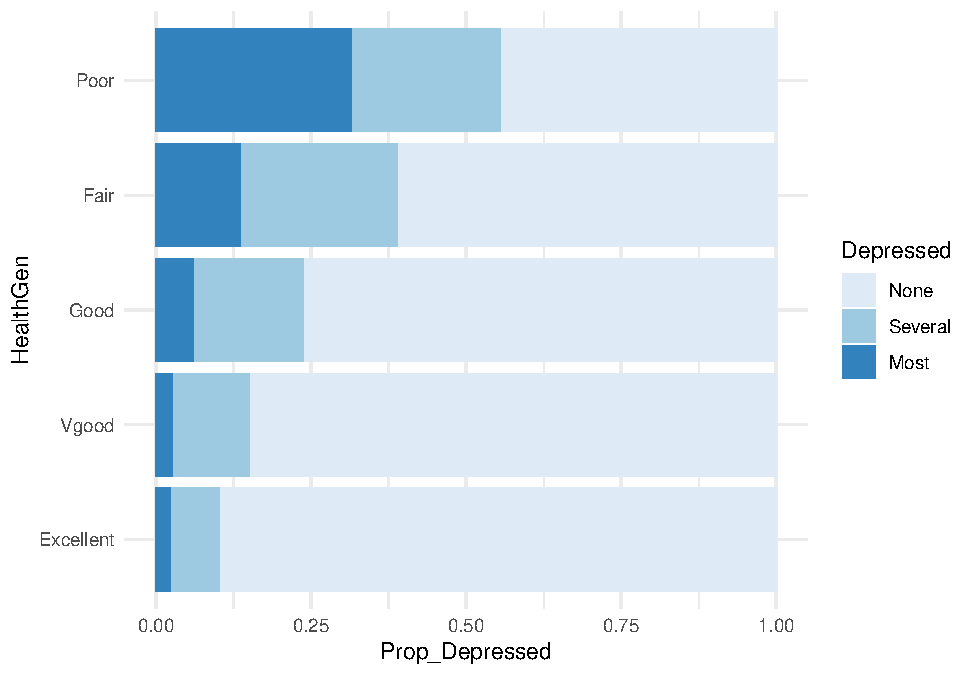
\includegraphics{_main_files/figure-latex/unnamed-chunk-44-1.pdf}

Perform a chi-square test of independence on contingency tables using the \texttt{svychisq()} function. Here is a test ofthe null hypothesis that depression is independent of general health.

\begin{Shaded}
\begin{Highlighting}[]
\FunctionTok{svychisq}\NormalTok{(}\SpecialCharTok{\textasciitilde{}}\NormalTok{Depressed }\SpecialCharTok{+}\NormalTok{ HealthGen, }\AttributeTok{design =}\NormalTok{ NHANES\_design, }\AttributeTok{statistic =} \StringTok{"Chisq"}\NormalTok{)}
\end{Highlighting}
\end{Shaded}

\begin{verbatim}
## 
##  Pearson's X^2: Rao & Scott adjustment
## 
## data:  svychisq(~Depressed + HealthGen, design = NHANES_design, statistic = "Chisq")
## X-squared = 1592.7, df = 8, p-value < 2.2e-16
\end{verbatim}

The chi-square test with Rao \& Scott adjustment is evidently not a standard chi-square test. \emph{Maybe in how it factors in survey design?} The test statistic is usually \(X^2 = \sum (O - E)^2 / E.\)

\begin{Shaded}
\begin{Highlighting}[]
\NormalTok{O }\OtherTok{\textless{}{-}} \FunctionTok{svytable}\NormalTok{(}\SpecialCharTok{\textasciitilde{}}\NormalTok{Depressed }\SpecialCharTok{+}\NormalTok{ HealthGen, }\AttributeTok{design =}\NormalTok{ NHANES\_design) }\SpecialCharTok{\%\textgreater{}\%} \FunctionTok{as.matrix}\NormalTok{()}
\NormalTok{E }\OtherTok{\textless{}{-}} \FunctionTok{sum}\NormalTok{(O) }\SpecialCharTok{*} \FunctionTok{prop.table}\NormalTok{(O, }\DecValTok{1}\NormalTok{) }\SpecialCharTok{*} \FunctionTok{prop.table}\NormalTok{(O, }\DecValTok{2}\NormalTok{)}
\NormalTok{(X2 }\OtherTok{\textless{}{-}} \FunctionTok{sum}\NormalTok{((O }\SpecialCharTok{{-}}\NormalTok{ E)}\SpecialCharTok{\^{}}\DecValTok{2} \SpecialCharTok{/}\NormalTok{ E))}
\DocumentationTok{\#\# [1] 16025254}
\FunctionTok{pchisq}\NormalTok{(X2, }\AttributeTok{df =}\NormalTok{ (}\FunctionTok{nrow}\NormalTok{(O)}\SpecialCharTok{{-}}\DecValTok{1}\NormalTok{) }\SpecialCharTok{*}\NormalTok{ (}\FunctionTok{ncol}\NormalTok{(O) }\SpecialCharTok{{-}} \DecValTok{1}\NormalTok{), }\AttributeTok{lower.tail =} \ConstantTok{FALSE}\NormalTok{)}
\DocumentationTok{\#\# [1] 0}
\end{Highlighting}
\end{Shaded}

which is what \texttt{chisq.test()} does.

\begin{Shaded}
\begin{Highlighting}[]
\FunctionTok{svytable}\NormalTok{(}\SpecialCharTok{\textasciitilde{}}\NormalTok{Depressed }\SpecialCharTok{+}\NormalTok{ HealthGen, }\AttributeTok{design =}\NormalTok{ NHANES\_design) }\SpecialCharTok{\%\textgreater{}\%} 
  \FunctionTok{as.matrix}\NormalTok{() }\SpecialCharTok{\%\textgreater{}\%} 
  \FunctionTok{chisq.test}\NormalTok{()}
\end{Highlighting}
\end{Shaded}

\begin{verbatim}
## 
##  Pearson's Chi-squared test
## 
## data:  .
## X-squared = 16025254, df = 8, p-value < 2.2e-16
\end{verbatim}

\hypertarget{exploring-quantitative-data}{%
\section{Exploring Quantitative Data}\label{exploring-quantitative-data}}

The \texttt{svymean()}, \texttt{svytotal()}, and \texttt{svyquantile()} functions summarize quantitative variables. To group by a factor variable, use \texttt{svyby()}.

\begin{Shaded}
\begin{Highlighting}[]
\FunctionTok{svyquantile}\NormalTok{(}\AttributeTok{x =} \SpecialCharTok{\textasciitilde{}}\NormalTok{SleepHrsNight, }
            \AttributeTok{design =}\NormalTok{ NHANES\_design, }
            \AttributeTok{na.rm =} \ConstantTok{TRUE}\NormalTok{, }
            \AttributeTok{quantiles =} \FunctionTok{c}\NormalTok{(.}\DecValTok{01}\NormalTok{, .}\DecValTok{25}\NormalTok{, .}\DecValTok{50}\NormalTok{, .}\DecValTok{75}\NormalTok{, .}\DecValTok{99}\NormalTok{))}
\end{Highlighting}
\end{Shaded}

\begin{verbatim}
## $SleepHrsNight
##      quantile ci.2.5 ci.97.5        se
## 0.01        4      4       5 0.2457588
## 0.25        6      6       7 0.2457588
## 0.5         7      7       8 0.2457588
## 0.75        8      8       9 0.2457588
## 0.99       10     10      11 0.2457588
## 
## attr(,"hasci")
## [1] TRUE
## attr(,"class")
## [1] "newsvyquantile"
\end{verbatim}

\begin{Shaded}
\begin{Highlighting}[]
\FunctionTok{svymean}\NormalTok{(}\AttributeTok{x =} \SpecialCharTok{\textasciitilde{}}\NormalTok{SleepHrsNight, }\AttributeTok{design =}\NormalTok{ NHANES\_design, }\AttributeTok{na.rm =} \ConstantTok{TRUE}\NormalTok{)}
\end{Highlighting}
\end{Shaded}

\begin{verbatim}
##                 mean     SE
## SleepHrsNight 6.9292 0.0166
\end{verbatim}

\begin{Shaded}
\begin{Highlighting}[]
\FunctionTok{svyby}\NormalTok{(}\AttributeTok{formula =} \SpecialCharTok{\textasciitilde{}}\NormalTok{SleepHrsNight, }\AttributeTok{by =} \SpecialCharTok{\textasciitilde{}}\NormalTok{Depressed, }\AttributeTok{FUN =}\NormalTok{ svymean, }
      \AttributeTok{design =}\NormalTok{ NHANES\_design, }\AttributeTok{na.rm =} \ConstantTok{TRUE}\NormalTok{, }\AttributeTok{keep.names =} \ConstantTok{FALSE}\NormalTok{) }\SpecialCharTok{\%\textgreater{}\%}
  \FunctionTok{ggplot}\NormalTok{(}\FunctionTok{aes}\NormalTok{(}\AttributeTok{x =}\NormalTok{ Depressed, }\AttributeTok{y =}\NormalTok{ SleepHrsNight, }
             \AttributeTok{ymin =}\NormalTok{ SleepHrsNight }\SpecialCharTok{{-}} \DecValTok{2}\SpecialCharTok{*}\NormalTok{se, }\AttributeTok{ymax =}\NormalTok{ SleepHrsNight }\SpecialCharTok{+} \DecValTok{2}\SpecialCharTok{*}\NormalTok{se)) }\SpecialCharTok{+}
  \FunctionTok{geom\_col}\NormalTok{(}\AttributeTok{fill =} \StringTok{"lightblue"}\NormalTok{) }\SpecialCharTok{+}
  \FunctionTok{geom\_errorbar}\NormalTok{(}\AttributeTok{width =} \FloatTok{0.5}\NormalTok{)}
\end{Highlighting}
\end{Shaded}

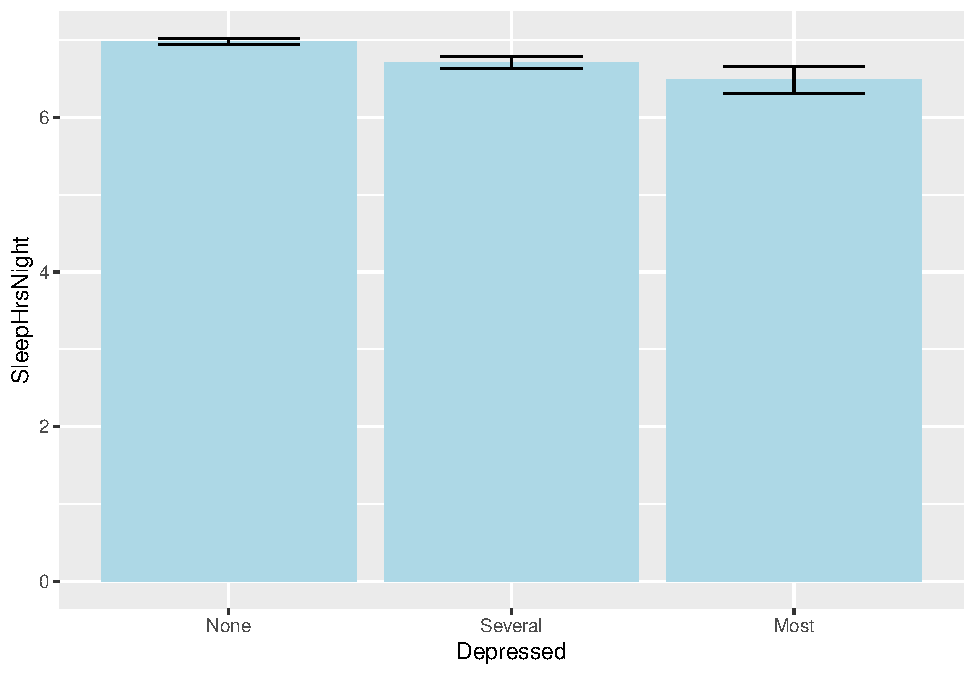
\includegraphics{_main_files/figure-latex/unnamed-chunk-49-1.pdf}

You need raw data for the distribution plots, so be sure to weight the variables.

\begin{Shaded}
\begin{Highlighting}[]
\NormalTok{NHANESraw }\SpecialCharTok{\%\textgreater{}\%} 
  \FunctionTok{ggplot}\NormalTok{(}\FunctionTok{aes}\NormalTok{(}\AttributeTok{x =}\NormalTok{ SleepHrsNight, }\AttributeTok{weight =}\NormalTok{ WTMEC4YR)) }\SpecialCharTok{+} 
  \FunctionTok{geom\_histogram}\NormalTok{(}\AttributeTok{binwidth =} \DecValTok{1}\NormalTok{, }\AttributeTok{fill =} \StringTok{"lightblue"}\NormalTok{, }\AttributeTok{color =} \StringTok{"\#FFFFFF"}\NormalTok{, }\AttributeTok{na.rm =} \ConstantTok{TRUE}\NormalTok{)}
\end{Highlighting}
\end{Shaded}

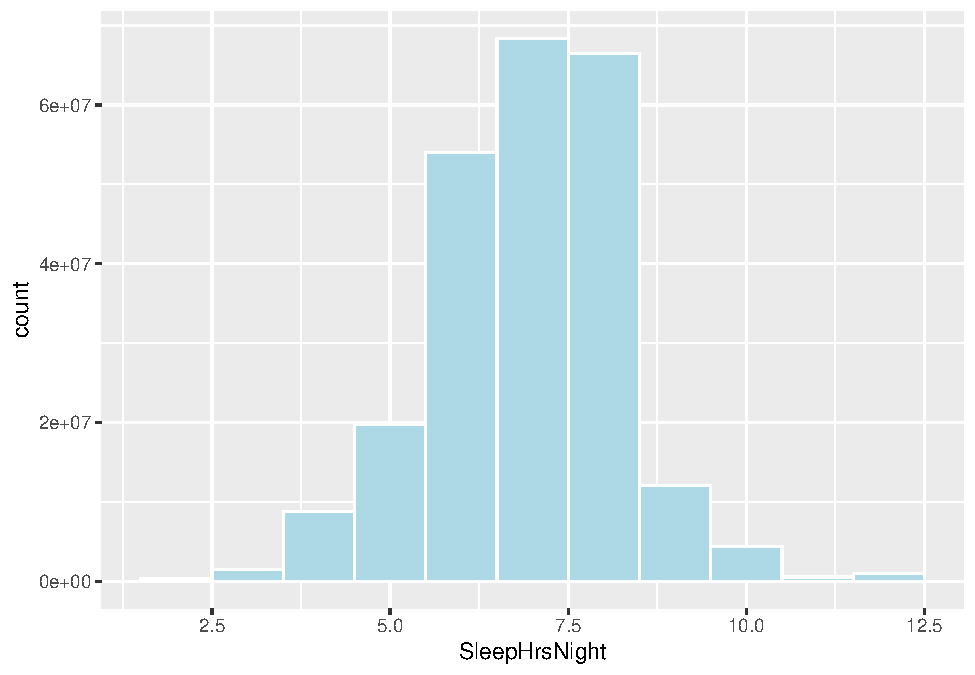
\includegraphics{_main_files/figure-latex/unnamed-chunk-50-1.pdf}

\begin{Shaded}
\begin{Highlighting}[]
\NormalTok{NHANESraw }\SpecialCharTok{\%\textgreater{}\%} 
  \FunctionTok{filter}\NormalTok{(}\SpecialCharTok{!}\FunctionTok{is.na}\NormalTok{(SleepHrsNight) }\SpecialCharTok{\&} \SpecialCharTok{!}\FunctionTok{is.na}\NormalTok{(Gender)) }\SpecialCharTok{\%\textgreater{}\%}
  \FunctionTok{group\_by}\NormalTok{(Gender) }\SpecialCharTok{\%\textgreater{}\%}
  \FunctionTok{mutate}\NormalTok{(}\AttributeTok{WTMEC4YR\_std =}\NormalTok{ WTMEC4YR }\SpecialCharTok{/} \FunctionTok{sum}\NormalTok{(WTMEC4YR)) }\SpecialCharTok{\%\textgreater{}\%}
  \FunctionTok{ggplot}\NormalTok{(}\FunctionTok{aes}\NormalTok{(}\AttributeTok{x =}\NormalTok{ SleepHrsNight, }\AttributeTok{Weight =}\NormalTok{ WTMEC4YR\_std)) }\SpecialCharTok{+}
  \FunctionTok{geom\_density}\NormalTok{(}\AttributeTok{bw =} \FloatTok{0.6}\NormalTok{, }\AttributeTok{fill =} \StringTok{"lightblue"}\NormalTok{) }\SpecialCharTok{+}
  \FunctionTok{labs}\NormalTok{(}\AttributeTok{x =} \StringTok{"Sleep Hours per Night"}\NormalTok{) }\SpecialCharTok{+}
  \FunctionTok{facet\_wrap}\NormalTok{(}\SpecialCharTok{\textasciitilde{}}\NormalTok{Gender, }\AttributeTok{labeller =} \StringTok{"label\_both"}\NormalTok{)}
\end{Highlighting}
\end{Shaded}

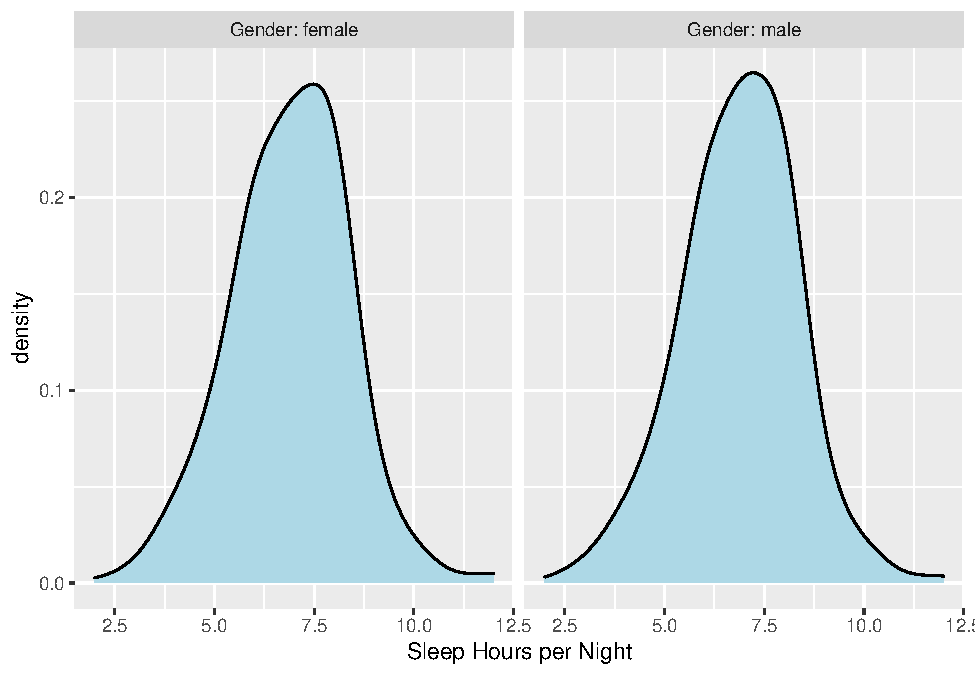
\includegraphics{_main_files/figure-latex/unnamed-chunk-50-2.pdf}

Test whether the population averages differ with a two-sample survey-weighted t-test. Use the \texttt{svytest()} function to incorporate the survey design.

\begin{Shaded}
\begin{Highlighting}[]
\FunctionTok{svyttest}\NormalTok{(}\AttributeTok{formula =}\NormalTok{ SleepHrsNight }\SpecialCharTok{\textasciitilde{}}\NormalTok{ Gender, }\AttributeTok{design =}\NormalTok{ NHANES\_design)}
\end{Highlighting}
\end{Shaded}

\begin{verbatim}
## Warning in summary.glm(g): observations with zero weight not used for
## calculating dispersion
\end{verbatim}

\begin{verbatim}
## Warning in summary.glm(glm.object): observations with zero weight not used for
## calculating dispersion
\end{verbatim}

\begin{verbatim}
## 
##  Design-based t-test
## 
## data:  SleepHrsNight ~ Gender
## t = -3.4077, df = 32, p-value = 0.001785
## alternative hypothesis: true difference in mean is not equal to 0
## 95 percent confidence interval:
##  -0.15506427 -0.03904047
## sample estimates:
## difference in mean 
##        -0.09705237
\end{verbatim}

\hypertarget{modeling-quantitative-data}{%
\section{Modeling Quantitative Data}\label{modeling-quantitative-data}}

Scatterplots need to adjust for the sampling weights. You can do this with the \texttt{size} or \texttt{alpha} aesthetics.

\begin{Shaded}
\begin{Highlighting}[]
\NormalTok{p1 }\OtherTok{\textless{}{-}}\NormalTok{ NHANESraw }\SpecialCharTok{\%\textgreater{}\%} 
  \FunctionTok{filter}\NormalTok{(Age }\SpecialCharTok{==} \DecValTok{20}\NormalTok{) }\SpecialCharTok{\%\textgreater{}\%}
  \FunctionTok{ggplot}\NormalTok{(}\FunctionTok{aes}\NormalTok{(}\AttributeTok{x =}\NormalTok{ Height, }\AttributeTok{y =}\NormalTok{ Weight, }\AttributeTok{color =}\NormalTok{ Gender, }\AttributeTok{size =}\NormalTok{ WTMEC4YR)) }\SpecialCharTok{+}
  \FunctionTok{geom\_jitter}\NormalTok{(}\AttributeTok{width =} \FloatTok{0.3}\NormalTok{, }\AttributeTok{height =} \DecValTok{0}\NormalTok{, }\AttributeTok{alpha =} \FloatTok{0.3}\NormalTok{) }\SpecialCharTok{+}
  \FunctionTok{guides}\NormalTok{(}\AttributeTok{size =} \ConstantTok{FALSE}\NormalTok{) }\SpecialCharTok{+}
  \FunctionTok{theme}\NormalTok{(}\AttributeTok{legend.position =} \StringTok{"top"}\NormalTok{) }\SpecialCharTok{+}
  \FunctionTok{labs}\NormalTok{(}\AttributeTok{color =} \StringTok{""}\NormalTok{)}
\end{Highlighting}
\end{Shaded}

\begin{verbatim}
## Warning: `guides(<scale> = FALSE)` is deprecated. Please use `guides(<scale> =
## "none")` instead.
\end{verbatim}

\begin{Shaded}
\begin{Highlighting}[]
\NormalTok{p2 }\OtherTok{\textless{}{-}}\NormalTok{ NHANESraw }\SpecialCharTok{\%\textgreater{}\%} 
  \FunctionTok{filter}\NormalTok{(Age }\SpecialCharTok{==} \DecValTok{20}\NormalTok{) }\SpecialCharTok{\%\textgreater{}\%}
  \FunctionTok{ggplot}\NormalTok{(}\FunctionTok{aes}\NormalTok{(}\AttributeTok{x =}\NormalTok{ Height, }\AttributeTok{y =}\NormalTok{ Weight, }\AttributeTok{color =}\NormalTok{ Gender, }\AttributeTok{alpha =}\NormalTok{ WTMEC4YR)) }\SpecialCharTok{+}
  \FunctionTok{geom\_jitter}\NormalTok{(}\AttributeTok{width =} \FloatTok{0.3}\NormalTok{, }\AttributeTok{height =} \DecValTok{0}\NormalTok{) }\SpecialCharTok{+}
  \FunctionTok{guides}\NormalTok{(}\AttributeTok{alpha =} \ConstantTok{FALSE}\NormalTok{) }\SpecialCharTok{+}
  \FunctionTok{theme}\NormalTok{(}\AttributeTok{legend.position =} \StringTok{"top"}\NormalTok{) }\SpecialCharTok{+}
  \FunctionTok{labs}\NormalTok{(}\AttributeTok{color =} \StringTok{""}\NormalTok{)}
\end{Highlighting}
\end{Shaded}

\begin{verbatim}
## Warning: `guides(<scale> = FALSE)` is deprecated. Please use `guides(<scale> =
## "none")` instead.
\end{verbatim}

\begin{Shaded}
\begin{Highlighting}[]
\NormalTok{gridExtra}\SpecialCharTok{::}\FunctionTok{grid.arrange}\NormalTok{(p1, p2, }\AttributeTok{nrow =} \DecValTok{1}\NormalTok{)}
\end{Highlighting}
\end{Shaded}

\begin{verbatim}
## Warning: Removed 4 rows containing missing values (geom_point).
\end{verbatim}

\begin{verbatim}
## Warning: Removed 4 rows containing missing values (geom_point).
\end{verbatim}

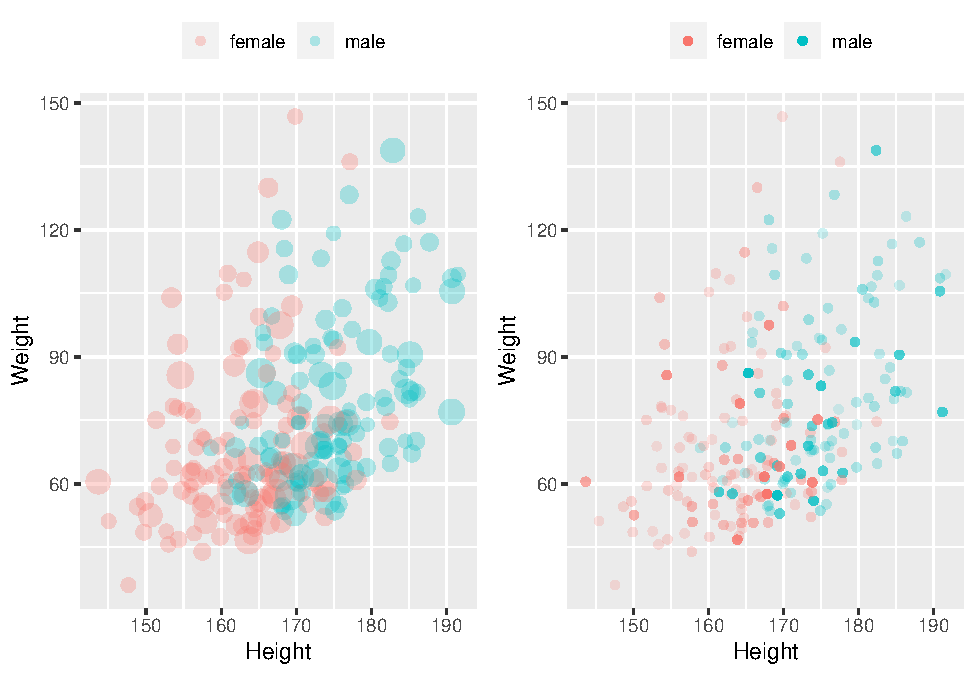
\includegraphics{_main_files/figure-latex/unnamed-chunk-52-1.pdf}

Fit a regression line with \texttt{geom\_smooth()}.

\begin{Shaded}
\begin{Highlighting}[]
\NormalTok{NHANESraw }\SpecialCharTok{\%\textgreater{}\%} 
  \FunctionTok{filter}\NormalTok{(}\SpecialCharTok{!}\FunctionTok{is.na}\NormalTok{(Weight) }\SpecialCharTok{\&} \SpecialCharTok{!}\FunctionTok{is.na}\NormalTok{(Height)) }\SpecialCharTok{\%\textgreater{}\%}
  \FunctionTok{ggplot}\NormalTok{(}\FunctionTok{aes}\NormalTok{(}\AttributeTok{x =}\NormalTok{ Height, }\AttributeTok{y =}\NormalTok{ Weight, }\AttributeTok{size =}\NormalTok{ WTMEC4YR)) }\SpecialCharTok{+}
  \FunctionTok{geom\_point}\NormalTok{(}\AttributeTok{alpha =} \FloatTok{0.1}\NormalTok{) }\SpecialCharTok{+}
  \FunctionTok{geom\_smooth}\NormalTok{(}\AttributeTok{method =} \StringTok{"lm"}\NormalTok{, }\AttributeTok{se =} \ConstantTok{FALSE}\NormalTok{, }\AttributeTok{mapping =} \FunctionTok{aes}\NormalTok{(}\AttributeTok{weight =}\NormalTok{ WTMEC4YR), }
              \AttributeTok{formula =}\NormalTok{ y }\SpecialCharTok{\textasciitilde{}}\NormalTok{ x, }\AttributeTok{color =} \StringTok{"blue"}\NormalTok{) }\SpecialCharTok{+}
  \FunctionTok{geom\_smooth}\NormalTok{(}\AttributeTok{method =} \StringTok{"lm"}\NormalTok{, }\AttributeTok{se =} \ConstantTok{FALSE}\NormalTok{, }\AttributeTok{mapping =} \FunctionTok{aes}\NormalTok{(}\AttributeTok{weight =}\NormalTok{ WTMEC4YR), }
              \AttributeTok{formula =}\NormalTok{ y }\SpecialCharTok{\textasciitilde{}} \FunctionTok{poly}\NormalTok{(x, }\DecValTok{2}\NormalTok{), }\AttributeTok{color =} \StringTok{"orange"}\NormalTok{) }\SpecialCharTok{+}
  \FunctionTok{geom\_smooth}\NormalTok{(}\AttributeTok{method =} \StringTok{"lm"}\NormalTok{, }\AttributeTok{se =} \ConstantTok{FALSE}\NormalTok{, }\AttributeTok{mapping =} \FunctionTok{aes}\NormalTok{(}\AttributeTok{weight =}\NormalTok{ WTMEC4YR), }
              \AttributeTok{formula =}\NormalTok{ y }\SpecialCharTok{\textasciitilde{}} \FunctionTok{poly}\NormalTok{(x, }\DecValTok{3}\NormalTok{), }\AttributeTok{color =} \StringTok{"red"}\NormalTok{) }\SpecialCharTok{+}
\FunctionTok{guides}\NormalTok{(}\AttributeTok{size =} \ConstantTok{FALSE}\NormalTok{) }
\end{Highlighting}
\end{Shaded}

\begin{verbatim}
## Warning: `guides(<scale> = FALSE)` is deprecated. Please use `guides(<scale> =
## "none")` instead.
\end{verbatim}

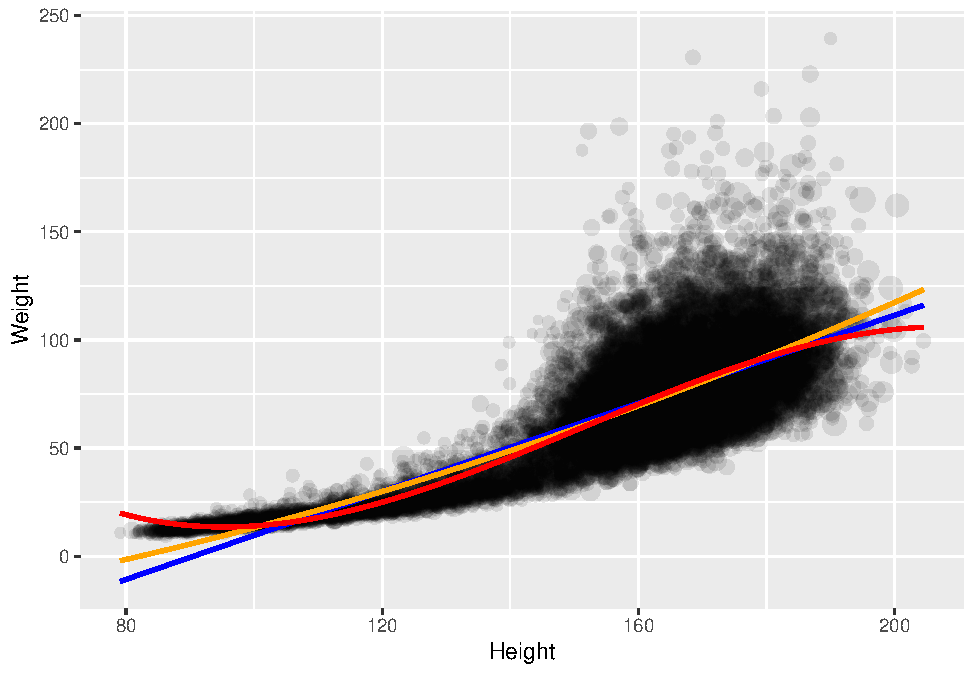
\includegraphics{_main_files/figure-latex/unnamed-chunk-53-1.pdf}

Model a regression line with \texttt{svyglm()}. Let's build a model to predict, BPSysAve, a person's systolic blood pressure reading, using BPDiaAve, a person's diastolic blood pressure reading and Diabetes, whether or not they were diagnosed with diabetes.

\begin{Shaded}
\begin{Highlighting}[]
\FunctionTok{drop\_na}\NormalTok{(NHANESraw, Diabetes, BPDiaAve, BPSysAve) }\SpecialCharTok{\%\textgreater{}\%}
\FunctionTok{ggplot}\NormalTok{(}\AttributeTok{mapping =} \FunctionTok{aes}\NormalTok{(}\AttributeTok{x =}\NormalTok{ BPDiaAve, }\AttributeTok{y =}\NormalTok{ BPSysAve, }\AttributeTok{size =}\NormalTok{ WTMEC4YR, }\AttributeTok{color =}\NormalTok{ Diabetes)) }\SpecialCharTok{+} 
    \FunctionTok{geom\_point}\NormalTok{(}\AttributeTok{alpha =} \FloatTok{0.2}\NormalTok{) }\SpecialCharTok{+} 
    \FunctionTok{guides}\NormalTok{(}\AttributeTok{size =} \ConstantTok{FALSE}\NormalTok{) }\SpecialCharTok{+} 
    \FunctionTok{geom\_smooth}\NormalTok{(}\AttributeTok{method =} \StringTok{"lm"}\NormalTok{, }\AttributeTok{formula =}\NormalTok{ y }\SpecialCharTok{\textasciitilde{}}\NormalTok{ x, }\AttributeTok{se =} \ConstantTok{FALSE}\NormalTok{, }\AttributeTok{mapping =} \FunctionTok{aes}\NormalTok{(}\AttributeTok{weight =}\NormalTok{ WTMEC4YR))}
\end{Highlighting}
\end{Shaded}

\begin{verbatim}
## Warning: `guides(<scale> = FALSE)` is deprecated. Please use `guides(<scale> =
## "none")` instead.
\end{verbatim}

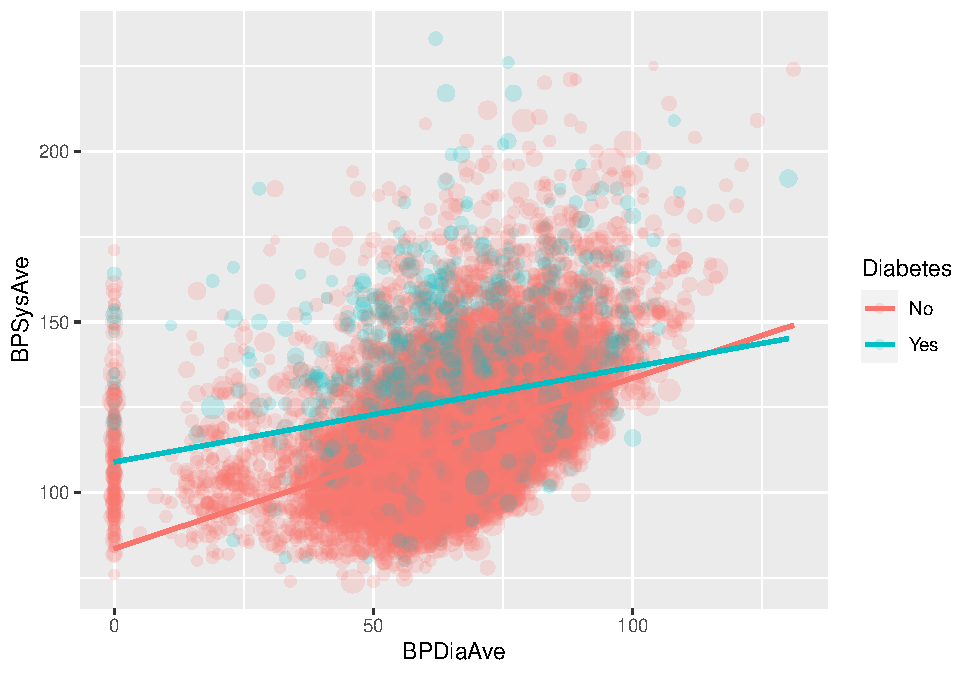
\includegraphics{_main_files/figure-latex/unnamed-chunk-54-1.pdf}

\begin{Shaded}
\begin{Highlighting}[]
\NormalTok{mod }\OtherTok{\textless{}{-}} \FunctionTok{svyglm}\NormalTok{(BPSysAve }\SpecialCharTok{\textasciitilde{}}\NormalTok{ BPDiaAve}\SpecialCharTok{*}\NormalTok{Diabetes, }\AttributeTok{design =}\NormalTok{ NHANES\_design)}
\FunctionTok{summary}\NormalTok{(mod)}
\end{Highlighting}
\end{Shaded}

\begin{verbatim}
## 
## Call:
## svyglm(formula = BPSysAve ~ BPDiaAve * Diabetes, design = NHANES_design)
## 
## Survey design:
## svydesign(data = NHANESraw, strata = ~SDMVSTRA, ids = ~SDMVPSU, 
##     nest = TRUE, weights = ~WTMEC4YR)
## 
## Coefficients:
##                      Estimate Std. Error t value Pr(>|t|)    
## (Intercept)          83.58652    2.05537  40.667  < 2e-16 ***
## BPDiaAve              0.49964    0.02623  19.047  < 2e-16 ***
## DiabetesYes          25.36616    3.56587   7.114 6.53e-08 ***
## BPDiaAve:DiabetesYes -0.22132    0.05120  -4.323 0.000156 ***
## ---
## Signif. codes:  0 '***' 0.001 '**' 0.01 '*' 0.05 '.' 0.1 ' ' 1
## 
## (Dispersion parameter for gaussian family taken to be 279.1637)
## 
## Number of Fisher Scoring iterations: 2
\end{verbatim}

\hypertarget{simple}{%
\chapter{Simple Random Samples}\label{simple}}

A simple random sample of size \emph{n} from a population of size \emph{N} has sampling weights are equal to \emph{N/n}. The Horvitz-Thompson estimator of the population sum for variable \emph{X} is

\[\hat{T}_X = \sum_{i=1}^n \check{X}_i = \frac{N}{n} \sum_{i=1}^n X_i\]

The variance of the estimator is

\[\mathrm{var} [\hat{T}_X] = \frac{N - n}{N} \times N^2 \times \frac{\mathrm{var}[X]}{n}\]

The first term in the variance is the \emph{finite population correction}. The third term is the vriance of the mean. The second term, \(N^2\), scales the mean to the total.

The estimator of the population mean is just the sum divided by \emph{N}.

\[\hat{\mu}_X = \hat{T}_X / N\]
and the variance of the mean is the unscaled population sum variance.

\[\hat{\mathrm{var}}[\hat{\mu}_X] = \mathrm{var} [\hat{T}_X] / N^2\]

\hypertarget{example}{%
\subsubsection*{Example}\label{example}}
\addcontentsline{toc}{subsubsection}{Example}

Data set \texttt{apisrs} is a simple random sample of the Academic Performance Index (API) of \emph{n} = 200 of the \emph{N} = 6,194 schools in California.

All \textbf{survey} objects require that you specify the columns identifying the clusters from largest to smallest level. In simple random designs like this, there are no clusters, and you specify just the constant \texttt{id\ =\ \textasciitilde{}1}. The \texttt{fpc} parameter specifies the column with the finite population correction. In a simple random sample, it equals \emph{N}. The \texttt{fpc} functions to both adjust the variance estimate, and to set the observation weights.

\begin{Shaded}
\begin{Highlighting}[]
\NormalTok{srs\_design }\OtherTok{\textless{}{-}} \FunctionTok{svydesign}\NormalTok{(}\AttributeTok{id =} \SpecialCharTok{\textasciitilde{}}\DecValTok{1}\NormalTok{,  }\AttributeTok{fpc =} \SpecialCharTok{\textasciitilde{}}\NormalTok{fpc, }\AttributeTok{data =}\NormalTok{ apisrs)}
\end{Highlighting}
\end{Shaded}

\(\hat{T}_X\), \(\mathrm{var} [\hat{T}_X]\), \(\hat{\mu}_X\), and \(\hat{\mathrm{var}}[\hat{\mu}_X]\) are

\begin{Shaded}
\begin{Highlighting}[]
\FunctionTok{svytotal}\NormalTok{(}\SpecialCharTok{\textasciitilde{}}\NormalTok{enroll, srs\_design)}
\DocumentationTok{\#\#          total     SE}
\DocumentationTok{\#\# enroll 3621074 169520}
\FunctionTok{svymean}\NormalTok{(}\SpecialCharTok{\textasciitilde{}}\NormalTok{enroll, srs\_design)}
\DocumentationTok{\#\#          mean     SE}
\DocumentationTok{\#\# enroll 584.61 27.368}
\end{Highlighting}
\end{Shaded}

When the sample is much smaller than the population, the finite population correction makes little difference. You can omit the \texttt{fpc} parameter, but then you must supply the samplying weight instead. In this case, the sampling weight is 200/6194, and is in variable \texttt{pw}. The total and mean are unchanged, but the variance increases a little without the correction.

\begin{Shaded}
\begin{Highlighting}[]
\NormalTok{srs\_design2 }\OtherTok{\textless{}{-}} \FunctionTok{svydesign}\NormalTok{(}\AttributeTok{id =} \SpecialCharTok{\textasciitilde{}}\DecValTok{1}\NormalTok{, }\AttributeTok{weights =} \SpecialCharTok{\textasciitilde{}}\NormalTok{pw, }\AttributeTok{data =}\NormalTok{ apisrs)}
\FunctionTok{svytotal}\NormalTok{(}\SpecialCharTok{\textasciitilde{}}\NormalTok{enroll, srs\_design2)}
\DocumentationTok{\#\#          total     SE}
\DocumentationTok{\#\# enroll 3621074 172325}
\FunctionTok{svymean}\NormalTok{(}\SpecialCharTok{\textasciitilde{}}\NormalTok{enroll, srs\_design2)}
\DocumentationTok{\#\#          mean     SE}
\DocumentationTok{\#\# enroll 584.61 27.821}
\end{Highlighting}
\end{Shaded}

\hypertarget{stratified}{%
\chapter{Stratified Sampling}\label{stratified}}

Stratified sampling is more common than simple random sampling because it is just as precise and costs less. Stratified sampling randomly samples from pre-defined groups (strata).

The Horvitz-Thompson estimator of the total is sum of the individual strati and its variance is the sum of the strati variances.

\hypertarget{example-1}{%
\subsubsection*{Example}\label{example-1}}
\addcontentsline{toc}{subsubsection}{Example}

Data set \texttt{apistrat} is a staratified sample of the Academic Performance Index (API) of \emph{n} = 200 of the \emph{N} = 6,194 schools in California. The strati are \(n_E\) = 100 elementary schools \(n_M\) = 50 middle schools, and \(n_H\) = 50 high schools. The \texttt{fpc} columnn in this data set is the population size \emph{for each stratum}.

\begin{Shaded}
\begin{Highlighting}[]
\NormalTok{strata\_design }\OtherTok{\textless{}{-}} \FunctionTok{svydesign}\NormalTok{(}\AttributeTok{id =} \SpecialCharTok{\textasciitilde{}}\DecValTok{1}\NormalTok{, }\AttributeTok{strata =} \SpecialCharTok{\textasciitilde{}}\NormalTok{stype, }\AttributeTok{fpc =} \SpecialCharTok{\textasciitilde{}}\NormalTok{fpc, }\AttributeTok{data =}\NormalTok{ apistrat)}
\FunctionTok{svytotal}\NormalTok{(}\SpecialCharTok{\textasciitilde{}}\NormalTok{stype, strata\_design)}
\end{Highlighting}
\end{Shaded}

\begin{verbatim}
##        total SE
## stypeE  4421  0
## stypeH   755  0
## stypeM  1018  0
\end{verbatim}

Since high schools tend to be larger, fixing the number of of sampled high schools should reduce the variance in mean and total enrollment relative to simple random sampling (compare to \texttt{apisrd} in Chapter \ref{simple}).

\begin{Shaded}
\begin{Highlighting}[]
\FunctionTok{svytotal}\NormalTok{(}\SpecialCharTok{\textasciitilde{}}\NormalTok{enroll, strata\_design)}
\DocumentationTok{\#\#          total     SE}
\DocumentationTok{\#\# enroll 3687178 114642}
\FunctionTok{svymean}\NormalTok{(}\SpecialCharTok{\textasciitilde{}}\NormalTok{enroll, strata\_design)}
\DocumentationTok{\#\#          mean     SE}
\DocumentationTok{\#\# enroll 595.28 18.509}
\end{Highlighting}
\end{Shaded}

\hypertarget{parts}{%
\chapter{Parts}\label{parts}}

You can add parts to organize one or more book chapters together. Parts can be inserted at the top of an .Rmd file, before the first-level chapter heading in that same file.

Add a numbered part: \texttt{\#\ (PART)\ Act\ one\ \{-\}} (followed by \texttt{\#\ A\ chapter})

Add an unnumbered part: \texttt{\#\ (PART\textbackslash{}*)\ Act\ one\ \{-\}} (followed by \texttt{\#\ A\ chapter})

Add an appendix as a special kind of un-numbered part: \texttt{\#\ (APPENDIX)\ Other\ stuff\ \{-\}} (followed by \texttt{\#\ A\ chapter}). Chapters in an appendix are prepended with letters instead of numbers.

\hypertarget{footnotes-and-citations}{%
\chapter{Footnotes and citations}\label{footnotes-and-citations}}

\hypertarget{footnotes}{%
\section{Footnotes}\label{footnotes}}

Footnotes are put inside the square brackets after a caret \texttt{\^{}{[}{]}}. Like this one \footnote{This is a footnote.}.

\hypertarget{citations}{%
\section{Citations}\label{citations}}

Reference items in your bibliography file(s) using \texttt{@key}.

For example, we are using the \textbf{bookdown} package \citep{R-bookdown} (check out the last code chunk in index.Rmd to see how this citation key was added) in this sample book, which was built on top of R Markdown and \textbf{knitr} (this citation was added manually in an external file book.bib).
Note that the \texttt{.bib} files need to be listed in the index.Rmd with the YAML \texttt{bibliography} key.

The RStudio Visual Markdown Editor can also make it easier to insert citations: \url{https://rstudio.github.io/visual-markdown-editing/\#/citations}

\hypertarget{blocks}{%
\chapter{Blocks}\label{blocks}}

\hypertarget{equations}{%
\section{Equations}\label{equations}}

Here is an equation.

\begin{equation} 
  f\left(k\right) = \binom{n}{k} p^k\left(1-p\right)^{n-k}
  \label{eq:binom}
\end{equation}

You may refer to using \texttt{\textbackslash{}@ref(eq:binom)}, like see Equation \eqref{eq:binom}.

\hypertarget{theorems-and-proofs}{%
\section{Theorems and proofs}\label{theorems-and-proofs}}

Labeled theorems can be referenced in text using \texttt{\textbackslash{}@ref(thm:tri)}, for example, check out this smart theorem \ref{thm:tri}.

\begin{theorem}
\protect\hypertarget{thm:tri}{}\label{thm:tri}For a right triangle, if \(c\) denotes the \emph{length} of the hypotenuse
and \(a\) and \(b\) denote the lengths of the \textbf{other} two sides, we have
\[a^2 + b^2 = c^2\]
\end{theorem}

Read more here \url{https://bookdown.org/yihui/bookdown/markdown-extensions-by-bookdown.html}.

\hypertarget{callout-blocks}{%
\section{Callout blocks}\label{callout-blocks}}

The R Markdown Cookbook provides more help on how to use custom blocks to design your own callouts: \url{https://bookdown.org/yihui/rmarkdown-cookbook/custom-blocks.html}

\hypertarget{sharing-your-book}{%
\chapter{Sharing your book}\label{sharing-your-book}}

\hypertarget{publishing}{%
\section{Publishing}\label{publishing}}

HTML books can be published online, see: \url{https://bookdown.org/yihui/bookdown/publishing.html}

\hypertarget{pages}{%
\section{404 pages}\label{pages}}

By default, users will be directed to a 404 page if they try to access a webpage that cannot be found. If you'd like to customize your 404 page instead of using the default, you may add either a \texttt{\_404.Rmd} or \texttt{\_404.md} file to your project root and use code and/or Markdown syntax.

\hypertarget{metadata-for-sharing}{%
\section{Metadata for sharing}\label{metadata-for-sharing}}

Bookdown HTML books will provide HTML metadata for social sharing on platforms like Twitter, Facebook, and LinkedIn, using information you provide in the \texttt{index.Rmd} YAML. To setup, set the \texttt{url} for your book and the path to your \texttt{cover-image} file. Your book's \texttt{title} and \texttt{description} are also used.

This \texttt{gitbook} uses the same social sharing data across all chapters in your book- all links shared will look the same.

Specify your book's source repository on GitHub using the \texttt{edit} key under the configuration options in the \texttt{\_output.yml} file, which allows users to suggest an edit by linking to a chapter's source file.

Read more about the features of this output format here:

\url{https://pkgs.rstudio.com/bookdown/reference/gitbook.html}

Or use:

\begin{Shaded}
\begin{Highlighting}[]
\NormalTok{?bookdown}\SpecialCharTok{::}\NormalTok{gitbook}
\end{Highlighting}
\end{Shaded}


  \bibliography{book.bib,packages.bib}

\end{document}
